\chapter{A COMPARATIVE STUDY OF EVOLUTIONARY MODELS IN COATI} \label{ch:marginal}

%%%%%%%%%%%%%%%%%%%%%%%%%%%%%%%%%%%%%%%%%%%%%%%%%%%%%%%%%%%%%%%%%%%%%%%%%%%%%%%%
\section{Introduction}
% Brief importance of alignment.
Sequence alignment plays a pivotal role in most bioinformatic analyses by providing a fundamental framework for the analysis of evolution, the central driving force in biology \citep{aniba2010msa}. Computational biologists frequently address evolutionary questions such as phylogenetic inference, ancestral sequence reconstruction, identification of disease-associated mutations, and measurement of selection through the analyses of genomic data, which require the use of alignment inference \citep{sequence_alignment_rosenberg_2009}. Alignments of sequences are not observed directly and must be inferred from sequence data using algorithms. Specifically, a sequence alignment is a hypothesis of which characters in two or more sequences are related by common descent \citep{cartwright2006logarithmic}. Every stage within a genomics analysis pipeline is vulnerable to errors, including those that precede sequence alignments, such as DNA contamination, sequencing and assembly errors, or misannotations of genomes \citep{zhang2021taper}. Consequently, sequence aligners face the challenge of accounting for these artifacts to prevent uncorrected errors from producing misleading results in comparative and functional genomic studies \citep{estimates_schneider_2009,effect_fletcher_2010,hubisz2011error}.

% Talk about coati and its improved accuracy over other methods.
In the previous chapter, I presented COATi, a statistical pairwise aligner that understands and corrects common genomic artifacts. Unlike other statistical aligners, COATi is based on finite state transducers (FSTs) and harnesses the inherent properties of FSTs to model features of molecular evolution. COATi combines a reversible codon substitution model, an insertion-deletion (indel) model that understands gap phases and handles frameshifts, and a step that models sequencing base calling errors that can introduce early stop codons. Results show that COATi is more accurate than current tools when aligning protein-coding sequences, especially in the presence of artifacts such as early stop codons or frameshifts.

% Better algorithms and tools lead to discoveries.
% New tools are developed to achieve higher accuracy in performing necessary tasks.
% Due to the large amounts of data, current tools must be accurate and fast.
% With the deluxe of information available in genomics, accuracy, and speed are indispensable requirements.

The design and implementation of novel algorithms are instrumental in advancing scientific understanding and enabling groundbreaking discoveries. In the field of genomics, where the magnitude of data in modern analyses is staggering, accuracy and speed are crucial prerequisites for developing innovative methods. This necessity for efficiency is the motivation behind integrating an approximate evolutionary model into COATi. While the triplet model in COATi, with an FST-based alignment algorithm, outperforms other available tools in terms of accuracy, the computational complexity of its implementation can become a bottleneck when processing lengthy sequences. To address this challenge, I introduced a marginal approximation to the evolutionary model in the previous chapter. This approximation harnesses traditional dynamic programming techniques, enhancing the capabilities of COATi to meet the demands of modern genomics.

% The results for the marginal model are very close to the triplet model and better than the other aligners, but not as good.
% In this chapter, I investigate how good of an approximation the marginal model is and describe it in depth.

In the upcoming sections of this chapter, I examine the relationship between the approximate and triplet models. While results show both approaches perform significantly better than other aligners (as detailed in Appendix \ref{ch:alignpair-supplement}), here I provide a comprehensive description of the approximate models and clarify how well they estimate the triplet model through a detailed analysis of relevant metrics.


%%%%%%%%%%%%%%%%%%%%%%%%%%%%%%%%%%%%%%%%%%%%%%%%%%%%%%%%%%%%%%%%%%%%%%%%%%%%%%%%
\section{Materials}
\subsection{Indel Model}

% I developed the marginal model because the triplet model (Evolution FST) can't be implemented in a faster way.
The triplet model in COATi is created by composing three FSTs, each tailored to represent a specific process of molecular evolution (substitutions and indels) or designed for error correction (base calling error). Specifically, the indel FST models insertions and deletions and assumes that the length of each deleted or inserted region has a geometric distribution (Fig.~\ref{fig:indel-marginal}). In addition, contiguous indels are exclusively modeled by insertions preceding deletions, with a direct path from the insertion state (I) to the deletion state (D) through the intermediate state (W), while the reverse path (D to I) must go through the match state (M). This design choice effectively limits the number of equivalent alignments and results in a more efficient alignment for the triplet model. Notably, the order of contiguous indels (i.e., insertion followed by deletion or deletion followed by insertion) does not affect the alignment score in this model.

\begin{figure}[!ht]
    \centering
    \hspace*{-5em}\resizebox{1.05\textwidth}{!}{
    \definecolor{colorR}{RGB}{228,26,28}    % RED
\definecolor{colorB}{RGB}{55,126,184}   % BLUE
\definecolor{colorG}{RGB}{77,175,74}    % GREEN
\definecolor{colorP}{RGB}{152,78,163}   % PURPLE
\definecolor{colorO}{RGB}{255,127,0}    % ORANGE
\definecolor{colorY}{RGB}{255,255,51}   % YELLOW
\definecolor{colorBn}{RGB}{166,86,40}   % BROWN
\definecolor{colorPk}{RGB}{247,129,191} % PINK
\definecolor{colorGy}{RGB}{153,153,153} % GRAY

\tikzstyle{line}=[draw, -stealth', very thick]
\tikzstyle{block}=[circle,fill=colorB!50,on grid]
\tikzstyle{lab}=[]
\tikzstyle{w}=[lab,midway]
\tikzstyle{e}=[lab,midway,auto=false,fill=white,font=\scriptsize]

\begin{tikzpicture}[node distance=40mm, auto,
	dottedline/.style = {ultra thick, loosely dotted,shorten >=1mm, shorten <=1mm}]
%%% Legend

%%% Indel FST
\node[block,fill=colorG!50] (start1) {start};
\node[block,below=25mm of start1] (M1) {M};
\node[block,below=of M1] (I1) {U};
\node[block,right=of I1] (U1) {I};
\node[block,above=of U1] (W1) {W};
\node[block,above=of W1] (D1) {V};
\node[block,right=of D1] (V1) {D};
\node[block,right=of W1] (S1) {S};
\node[block,fill=colorR!50,right=25mm of S1] (end1) {end};

\draw (D1) +(0mm,-20mm) coordinate (C1);
\draw (D1) +(50mm,-10mm) coordinate (C2);

\draw[line] (start1) -- (M1);
\draw[line] (M1) -- node[w] {$g$} (I1);
\draw[line] (M1) -- node[w] {$1-g$} (W1);
\draw[line] (U1) to[out=150,in=30]  node[w,above] {$e$} (I1);
\draw[line] (U1) -- node[w,pos=0.1,right] {$1-e$} (W1);
\draw[line] (W1) -- node[w] {$g$} (D1);
\draw[line] (W1) -- node[w] {$1-g$} (S1);
\draw[line] (S1) -- node[w] {} (end1);
\draw[line] (V1) to[out=150,in=30] node[w,above] {$e$} (D1);
% \draw[line] (D1) to[out=60,in=90] node[w] {$1-e$} (end1 |- D1.south) to (end1);
\draw[line] (V1) -- node[w,swap] {$1-e$} (S1);


\draw[line] (I1) to[bend right=35] (U1);
\draw[line] (I1) to[bend right=30] (U1);
\draw[line] (I1) to[bend right=40] (U1);
\draw[line] (I1) to[bend right=25] node[e] {\O:Z/$\grande{\pi}_{\text{Z}}$} (U1);
% \draw[line] (I1) to[out=270, in=270] node[w,above=1mm] {$(1-e)(1-g)$} (end1 |- I1.south) to (end1);

\draw[line] (D1) to[bend right=25] (V1);
\draw[line] (D1) to[bend right=35] (V1);
\draw[line] (D1) to[bend right=30] (V1);
\draw[line] (D1) to[bend right=40] (V1);
\draw[line] (D1) to[bend right=20] node[e] {Y:\O} (V1);

\draw[line] (S1) to[bend left=42] (M1);
\draw[line] (S1) to[bend left=48] (M1);
\draw[line] (S1) to[bend left=45] (M1);
\draw[line] (S1) to[bend left=51] (M1);

\draw[line] (S1) to[bend left=39] node[e,pos=0.25] {Y:Z} (M1);

\node[font=\footnotesize,text width=50mm,below=7cm of start1] (sequences) {
\begin{tabular}{r@{\,: }l}
\multicolumn{2}{l}{\textbf{Sequences}}\\
    \hline
	% X & input nucleotides\\
	Y & intermediate nucleotides\\
	Z & output nucleotides\\
	\O & nothing/empty sequence\\
\end{tabular}
};

\node[font=\footnotesize,right=0.5cm of sequences,text width=50mm] {
\begin{tabular}{r@{\,: }l}
\multicolumn{2}{l}{\textbf{Parameters}}\\
\hline
	$g$ & gap open weight\\
	$e$ & gap extension weight\\
   	$\pi$ & nucleotide stationary frequency\\
\end{tabular}
};


\end{tikzpicture}
    }
    \caption[COATi Indel Model]{Indel FST for the triplet model. Allows insertions (U to I) and deletions (V to D). Insertion arcs are weighted by the corresponding nucleotide stationary frequency ($\pi$). The path and weight to the end state are designed so that the start and end gaps are symmetric. The arc weights are defined in linear space using gap opening ($g$) and gap extension ($e$) parameters. Arcs indicate an input symbol : output symbol / and weight. Missing symbols indicate no consumption or emission of symbols and missing weights indicate a weight of 1.}
    \label{fig:indel-marginal}
\end{figure}

Given the inherent characteristics of the triplet codon substitution model, the alignment can only be performed using FST-based algorithms, which can become costly for long pairs of sequences. To enhance COATi's data processing capacity and broaden its usability, I developed an approximate model that facilitates a faster alignment implementation. This is achieved by transforming the codon substitution probability matrix, thus allowing the reduction of the triplet model to a three-state FST (Fig.~\ref{fig:marginal-model}). This streamlined model preserves its original indel weights and is compatible with established pairwise dynamic programming methods.

\begin{figure}[!ht]
    \centering
    \resizebox{0.95\textwidth}{!}{
    
%\documentclass{article}
% \usepackage{pgf}
% \usepackage{tikz}
% \usetikzlibrary{arrows,automata,positioning,shapes}
% \usepackage{verbatim}
% \usepackage{graphicx}

\tikzset{
  font={\fontsize{9pt}{11}\selectfont}
}

\definecolor{colorR}{RGB}{228,26,28}    % RED
\definecolor{colorB}{RGB}{55,126,184}   % BLUE
\definecolor{colorG}{RGB}{77,175,74}    % GREEN
\definecolor{colorP}{RGB}{152,78,163}   % PURPLE
\definecolor{colorO}{RGB}{255,127,0}    % ORANGE
\definecolor{colorY}{RGB}{255,255,51}   % YELLOW
\definecolor{colorBn}{RGB}{166,86,40}   % BROWN
\definecolor{colorPk}{RGB}{247,129,191} % PINK
\definecolor{colorGy}{RGB}{153,153,153} % GRAY

\begin{tikzpicture}[->,>=stealth',shorten >=1pt,auto,node distance=7cm,ultra thick]
  \tikzstyle{every node}=[font=\large]

  \node[circle,fill=colorG!50,minimum size=1cm]  (S)					  {\textbf{Start}};
  \node[circle,fill=colorB!50,minimum size=1cm]  (M) [right=30mm of S]  {\textbf{M}};
  \node[circle,fill=colorB!50,minimum size=1cm]  (I) [above right of=M] {\textbf{I}};
  \node[circle,fill=colorR!50,minimum size=1cm]  (E) [below right of=M] {\textbf{End}};
  \node[circle,fill=colorB!50,minimum size=1cm]  (D) [below right of=I] {\textbf{D}};

  \path (S) edge 			  node {}	(M)
	(M) edge [out=265,in=200,looseness=10]  node [midway,font=\large] {$(1-g)^2 \cdot s$} (M)
  		edge [bend left]  node [font=\large] {$g$} (I)
            edge [out=10,in=170]  node [font=\large,pos=0.4] {$(1-g)\cdot g$} (D)
            edge [bend right] node [pos=0.35, rotate=-45, font=\large] {$(1-g)^2$}	(E)
        (I) edge [out=120,in=60,looseness=10] node [font=\large] {$e$} (I)
            edge [out=240,in=30]  node [rotate=50, above=1em, font=\large] {$(1-e)\cdot (1-g) \cdot s$} (M)
            edge [bend left]  node [pos=0.3, rotate=-45, right=1.75em, font=\large] {$(1-e) \cdot g $} (D)
            edge [bend left] node [pos=0.96, rotate=60, right=1.5em, font=\large] {$(1-e) \cdot (1-g)$} (E)
        (D) edge [out=30,in=330,looseness=10] node [font=\large] {$e$} (D)
            edge [out=190,in=-10]  node [below, font=\large, pos=0.6] {$(1-e) \cdot s$} (M)
            edge [bend left]  node [font=\large] {$1-e$} (E);

  \node[text width=4cm, below left=-10mm and 28mm of E, font=\bfseries] (parameters) {
  \begin{tabular}{r@{\,: }l}
  \multicolumn{2}{l}{\textbf{Parameters}}\\
    \hline
  $g$ & gap opening\\
  $e$ & gap extension\\
  $s$ & substitution\\
  \end{tabular}
  };

\end{tikzpicture}


    }
    \caption[Approximate Indel Model]{Approximate indel model, a three-state pairwise alignment architecture based on the Evolution FST described in COATi. Arcs to the match state (M) take and emit nucleotides based on a modified codon substitution model probability, whereas arcs to indel states introduce insertions (I) or deletions (D). The transition probabilities are defined in linear space and weighted using parameters gap opening (\textit{g}), gap extension (\textit{e}), and substitution ($s$).}
    \label{fig:marginal-model}
\end{figure}

% Explain in the previous chapter that we lose probability mass because we condition on starting and ending with a pseudo-match to simplify the model. Reminder here.

As described in the previous chapter, the triplet evolutionary FST model calculates the probability of a descendant sequence given an ancestral one, with parameters branch length, coefficient of selective pressure, and residue stationary frequencies. This probability is conditional on starting and ending the alignment with a pseudo-match to simplify the model and for start and end gaps to be symmetric, which results in the alignment weight being affected by a scaling factor. While this does not affect the ability of COATi to find the best alignment, this condition is inherited by the approximate model.

\subsection{Alignment and Semirings} %%%%%%%%%%%%%%%%%%%%%%%%%%%%%%%%%%%%%%%%%%%%
% two distinct alignment operations. However, both use semirings, more specifically the tropical semiring.
% To prevent underflow, we need to perform calculations in log space
% Because of that, the tropical semiring is perfect for implementing the Viterbi - times operator (plus) calculates transition probabilities between states, and the plus operator (max) chooses the best transition/step.
% By defining additional semiring types, coati also has a sampler algorithm that uses the intermediate values from the Forward algorithm, which runs using the log semiring.

% Let's try the opposite: generate a need for semirings, then introduce them.
% Alternative start: Statistical alignment finds the optimal path between two sequences (etc.).
Pairwise statistical alignment defines a probabilistic framework for finding the minimum cost or the most likely path through a state transition graph, where each state represents a position in two biological sequences, and each transition represents an evolutionary event (no substitution, substitution, insertion, or deletion). The optimal path corresponds to the most biologically meaningful alignment of the sequences under a specific model. Since the transition probabilities are generally less than one, their product can result in small numbers, especially when dealing with long DNA sequences. Due to the limitations of standard floating-point arithmetic in modern computers, this can lead to numerical underflow. When this occurs, the likelihood can become virtually zero, thus leading to incorrect results. To address this issue, calculations in statistical alignment algorithms are typically performed in logarithmic space, thus preventing underflow \citep{durbin1998biological}.

\begin{table}[!ht]
\centering
\begingroup\centering
\begin{tabular}{c||c|c|c|c|c}
Semiring & Set & $\oplus$ & $\otimes$ & $\overline{0}$ & $\overline{1}$\\
\hline\hline
Linear   & $ \mathbb{R}_+$ & $+$ & $\times$ & 0 & 1\\
Log      & $ \mathbb{R} \cup \{ -\infty, +\infty \}$ & $\oplus_{\text{log}}$ & + & -$\infty$ & 0\\
Tropical & $ \mathbb{R} \cup \{ -\infty, +\infty \}$ & max & + & -$\infty$ & 0\\
\end{tabular}
\par\endgroup
 \vspace{1mm}
 \caption[Semirings]{Types of semirings implemented in COATi and their defined operations.}
 \label{table:semiring}
\end{table}

% something to tie the need for log space to semirings and alignment in coati
% then talk about semirings briefly
COATi includes two alignment procedures, one based on FST operations for the triplet model and one based on Gotoh's \citeyearpar{gotoh_1982} algorithm for the approximate model (Appendix \ref{ch:ch3-supplement}). Despite having different implementations, both approaches perform their computations in logarithmic space through the use of semirings, either as included in the openFST library \citep{allauzen2007openfst} for the former or self-implemented for the latter. Mathematical semirings are algebraic structures that define two binary operations, usually denoted by addition ($\oplus$) and multiplication ($\otimes$). Addition behaves like a commutative monoid with identity element $\overline{0}$ ($a \oplus b = b \oplus a$ and $a \oplus \overline{0} = a$), while multiplication is distributed over addition ($a \otimes (b \oplus c) = (a \otimes b) \oplus (a \otimes c)$) and has an identity element $\overline{1}$ ($a \otimes \overline{1} = a$). In particular, the tropical semiring (Table \ref{table:semiring}) is ideal for implementing the Viterbi algorithm with logarithmic transition scores, which finds the best path through a sequence of states by calculating the score of each possible transition for each state using the $\otimes$ operator ($+$) and selects the optimal one with $\oplus$ (max). Both alignment procedures are implemented using the tropical semiring.

% % marginal model alignment
% The core algorithm for the marginal model is a flexible implementation of the Forward algorithm that supports running both the Forward and the Viterbi algorithms, thanks to C++ templates and semiring types. The Forward algorithm calculates the weight of all possible alignments and is run using the log semiring. COATi features a pairwise alignment sampler that uses all intermediate scores from the Forward algorithm \cyan{(coati sample - Appendix x)}. The tropical semiring runs the Viterbi algorithm, which finds the optimal path (alignment) between two sequences. The Viterbi algorithm is implemented using a version of the Gotoh \citeyearpar{gotoh_1982} algorithm modified to follow the transition probabilities between match, insertion, and deletion states of the marginal model (Algo. \ref{alg:alignpair}).

% \begin{algorithm}[hp]
% forward_impl from coati with gap unit length = 1
\setstretch{1.1}
\begin{algorithmic}[1]
\Function{alignpair}{$s$, $v$, $g$, $e$}
  \State $n, m \gets |s|, |v|$
  \State $\text{M, D, I} \gets \operatorname{zero}(n+1, m+1)$ \Comment{Initialize the matrices of size $n+1$ by $m+1$}
  \For{$i \gets 1$ to $n$} \Comment{Gap deletion penalties}
    \State $\text{D}[i, 0] \gets g \oplus ((i - 1) \otimes e)$
  \EndFor
  \For{$j \gets 1$ to $m$} \Comment{Gap insertion penalties}
    \State $\text{I}[0, j] \gets g \oplus ((j - 1) \otimes e)$
  \EndFor
  \State $M[0,0] \gets \overline{1}$ \Comment{Set starting value in match matrix}

  \For{$i \gets 1$ to $n$} \Comment{Fill in the matrices}
    \For{$j \gets 1$ to $m$}
      % \State \textbf{Compute} match
      \State $\text{mch2mch} \gets M[i-1, j-1] \otimes \log_{1m} (g) \otimes \log_{1m} (g) \otimes \text{P}_{apx}[s_i, v_j]$
      \State $\text{del2mch} \gets D[i-1, j-1] \otimes \log_{1m} (e) \otimes \text{P}_{apx}[s_i, v_j]$
      \State $\text{ins2mch} \gets I[i-1, j-1] \otimes \log_{1m} (e) \otimes \log_{1m} (g) \otimes \text{P}_{apx}[s_i, v_j]$

      % \State \textbf{Compute} deletion
      \State $\text{mch2del} \gets M[i-1, j] \otimes \log_{1m} (g) \otimes g$
      \State $\text{del2del} \gets D[i-1, j] \otimes e$
      \State $\text{ins2del} \gets I[i-1, j] \otimes \log_{1m} (e) \otimes g$
      
      % \State \textbf{Compute} insertion
      \State $\text{mch2ins} \gets M[i, j-1] \otimes g$
      \State $\text{ins2ins} \gets I[i, j-1] \otimes e$
        
      \State $M[i, j] = \text{mch2mch} \oplus \text{del2mch} \oplus \text{ins2mch}$ \Comment{Save match scores}
      \State $D[i, j] = \text{mch2del} \oplus \text{del2del} \oplus \text{ins2del}$ \Comment{Save deletion scores}
      \State $I[i, j] = \text{mch2ins} \oplus \text{ins2ins}$ \Comment{Save insertion scores}

    \EndFor
  \EndFor
\State \textbf{Add end weights}
\State \textbf{Traceback}
\EndFunction
\end{algorithmic}
\caption[Marginal and Modal Alignment Pseudocode]{Marginal pairwise alignment algorithm. Intentionally different from the Gotoh algorithm to implement the marginal evolutionary model in COATi.}\label{alg:alignpair}
\end{algorithm}

% !!!!!!!!!!!!!!!!!!!!!!!! Moved to chapter 2 !!!!!!!!!!!!!!!!!!!!!!!!!!!!!!!!

% \subsection{Codon Substitution Models} %%%%%%%%%%%%%%%%%%%%%%%%%%%%%%%%%%%%%%%
% % Substitution model
% % Q matrix then marginal where, if following tropical semiring operators, max is the default option (tropical semiring). The Sum model is the alternative where we hypothesize is better (potential conflict since marginal-sum is the model used in the previous chapter).
% % Introduce MG94 and ECM from the ground up using the same definition for the instantaneous substitution matrix Q. Introduce every variable and be extremely precise about Q and P.

% % Conceptually, the essence of the approximation is to make the nucleotides on the descendant sequence independent of each other and only conditional on the ancestral codon and reading frame. The marginalization process is implemented for the mechanistic Muse and Gaut \citeyearpar{muse_gaut_1994} (MG94) and the Empirical Codon \citep{kosiol_ECM_2007} (ECM) models. In addition, COATi can read and marginalize a user-provided 61x61 codon substitution model.

% \subsubsection{Muse and Gaut}

% Codon substitution is particularly suitable for modeling protein-coding genes since it accounts for both the likelihood of mutations occurring at the nucleotide level and selective pressure on amino acid substitutions \citep{sullivan2005model}. While codon models are extensively applied to reconstruct phylogenies and study natural selection \citep{delport2009models}, their use in alignment reconstruction is still scarce. COATi is the only aligner that implements the mechanistic Muse and Gaut model (MG94), a codon model designed for coding regions \citep{muse_gaut_1994}. Modeled as a continuous-time Markov process, the instantaneous substitution rate matrix \textit{Q} defines the rate that codon \textit{X} changes to codon \textit{Y} as

% %  Q matrix MG94
% \begin{align}
% Q_{XY} &=  \begin{cases}
%     0 & \text{if $X$ and $Y$ differ by more than one nucleotide change}\\
%     \grande{\mu}_{X_pY_p} & \text{if $X$ and $Y$ are synonymous}\\
%     \omega \cdot \grande{\mu}_{X_pY_p} & \text{if $X$ and $Y$ are nonsynonymous}
% \end{cases}\\
% Q_{XX} &= -\sum_{Y:Y \neq X} Q_{XY}
% \end{align}
% where $X$ and $Y$ are non-stop codons defined $X,Y \in \grande{\Sigma}_{codon} - \{\text{TAA, TAG, TGA}\}$, $\omega$ is the strength of selection affecting amino-acid changes, and $X_p$ and $Y_p$ refer to the nucleotides in position \textit{p} in codons \textit{X} and \textit{Y} respectively, defined $X_p, Y_p \in \Sigma_{DNA}$. $\grande{\mu}_{X_pY_p}$ represents the mutation rate that nucleotide $X_p$ is replaced by $Y_p$ defined $\grande{\mu}_{X_pY_p} = \grande{\pi}_{Y_p} \grande{\sigma}_{X_pY_p}, \forall\ X_p \neq Y_p$, where $\grande{\pi}_{Y_p}$ is the equilibrium frequency of nucleotide $Y_p$, and $ \grande{\sigma}_{X_pY_p}$ corresponds to one of the instantaneous substitution parameters (Table \ref{table:gtr}) of the General Time Reversible nucleotide substitution model \citep{tavare_gtr_1986} (GTR). I use the nucleotide stationary frequencies and GTR parameters inferred from primate data by Yang \citeyear{yang1994estimating} to construct MG94 in COATi.

% The GTR model is a well-known and widely-used substitution model that allows variable instantaneous mutation rates between each of the six nucleotide pairs, with equal forward and reverse rates for any given pair. This property is represented
% $\grande{\pi}_{Y_p} \grande{\mu}_{X_pY_p} = \grande{\pi}_{X_p} \grande{\mu}_{Y_pX_p}$
% and transfers to the MG94 model,
% % $\grande{\pi}_Y Q_{XY} = \grande{\pi}_X Q_{YX}$
% making both models time-reversible.

% \begin{table}[!ht]
% \centering
% \begingroup\centering
\begin{tabular}{c||c|c|c|c}
& A & C & G & T\\
\hline\hline
A & $\ast$ & $\grande{\pi}_C \grande{\sigma}_{AC}$ & $\grande{\pi}_G \grande{\sigma}_{AG}$ & $\grande{\pi}_T \sigma_{AT}$\\
C & $\grande{\pi}_A \grande{\sigma}_{CA}$ & $\ast$ & $\grande{\pi}_G \grande{\sigma}_{CG}$ & $\grande{\pi}_T \sigma_{CT}$\\
G & $\grande{\pi}_A \grande{\sigma}_{GA}$ & $\grande{\pi}_C \grande{\sigma}_{GC}$ & $\ast$ & $\grande{\pi}_T \sigma_{GT}$\\
T & $\grande{\pi}_A \grande{\sigma}_{TA}$ & $\grande{\pi}_C \grande{\sigma}_{TC}$ & $\grande{\pi}_G \grande{\sigma}_{TG}$ & $\ast$\\
\end{tabular}
\par\endgroup
%  \vspace{2mm}
%  \caption[General Time Reversible Model]{Instantaneous nucleotide substitution rates for the General Time Reversible model (GTR). On each row, the parameters represent the probability of a given nucleotide being replaced by another. GTR is the most general and time-reversible nucleotide substitution model, with a different mutation rate parameter for each of the six possible nucleotide combinations. Note that sigma parameters for each of the six possible nucleotide pairs are identical (i.e., $\sigma_{AC} = \sigma_{CA}$, $\sigma_{AG} = \sigma_{GA}$, etc.).}
%  \label{table:gtr}
% \end{table}

% \subsubsection{Empirical Codon Model}

% In addition to the MG94 codon model, COATi incorporates an empirical codon model that can be used with the triplet and marginal alignment procedures. While mechanistic models explicitly account for molecular evolution features and use a defined set of parameters to specify them, empirical models, in contrast, attempt to summarize the substitution patterns inferred from extensive datasets. Although codon substitution models are rare in sequence aligners, the Empirical Codon Model (ECM) is the most common. This model is characterized by incorporating instantaneous doublet and triplet changes and encoding the physicochemical properties of amino acids \citep{kosiol_ECM_2007}. The ECM model was estimated using 7,332 protein families from the Pandit database, a collection of protein-coding multiple sequence alignments \citep{whelan2006pandit}. 

% Although purely empirical substitution models can be applied as is, the empirical codon model offers a combined approach with mechanistic parameters. Similar to the MG94 model definition, the instantaneous substitution rate matrix Q for the ECM model defines the rate that codon $X$ changes to codon $Y$ as
% % Q matrix ECM
% \begin{align}
% Q_{XY} &=  \begin{cases}
%     \grande{s}^*_{XY} \cdot \pi_Y & \text{if $X$ and $Y$ are synonymous}\\
%     \grande{s}^*_{XY} \cdot \pi_Y \cdot \omega & \text{if $X$ and $Y$ are nonsynonymous}
% \end{cases}\\
% Q_{XX} &= -\sum_{Y:Y \neq X} Q_{XY}
% \end{align}
% where $X$ and $Y$ are non-stop codons defined $X, Y \in \grande{\Sigma}_{codon} - \{\text{TAA, TAG, TGA}\}$, $\grande{s}^*_{XY}$ are the ECM exchangeabilities estimated from the Pandit database, and $\grande{\pi}$ is the frequency of codon $Y$. Note that this model is also time-reversible.

% For both MG94 and ECM, the probability that codon \textit{Y} replaces codon \textit{X} after time \textit{t} is calculated via matrix exponentiation: $P(Y|X; \Theta) = e^{Q_{XY}t}$, where $\Theta$ is the set of models parameters $\Theta_{MG} = \{t, \omega, \pi, \sigma\}$ for MG94 and $\Theta_{ECM} = \{t, \omega, \pi, s^* \}$ for ECM \citep{holmes2002expectation}. Note that as these models are applied in the context of protein-coding sequences, stop codons are not considered, resulting in a 61x61 matrix. In addition, probabilities are log-transformed to prevent underflow.

%% !!!!!!!!!!!!!!!!!!!!!!!!!!!!!!!!!!!!!!!!!!!!!!!!!!!!!!!!!!!!!!!!!!!!!!!!!!!

\subsection{Marginal Substitution Model} %%%%%%%%%%%%%%%%%%%%%%%%%%%%%%%%%%%%%%%

% Remember that we store marginal probabilities in log space.
% Intro sentence recalling the tropical semiring and marginalization (?).

% Speed up, MG94, why this particular marginalization - anc/des, tropical semiring(?).
% Conceptually, the essence of the approximation is to make the nucleotides on the descendant sequence independent of each other and only conditional on the ancestral codon and reading frame. T
I developed the approximate model to speed up the alignment in COATi. The main restriction of the triplet model that prevents its implementation using a dynamic programming approach is the nucleotide dependence in each pair of sequences, given by the substitution model. The triplet model is a 61 by 61 time-reversible codon substitution model described in the previous chapter \ref{ch:alignpair}. The approximation makes the nucleotides in each codon in the descendant sequence individually independent by calculating the probability that each ancestral codon produces specific descendant nucleotides at each reading frame position.

If we let $X= \{X_1 X_2 X_3\}$ and $Y = \{Y_1 Y_2 Y_3\}$ be codons from $\grande{\Sigma}_{codon}$, composed by nucleotides $\{X_1,X_2,X_3\} \in \grande{\Sigma}_{DNA}$ and $\{Y_1,Y_2,Y_3\} \in \grande{\Sigma}_{DNA}$ respectively, the probability that the descendant codon $Y$ substitutes the ancestral codon $X$ after time $t \in \Theta$ by the triplet model is $P\left(Y_1 Y_2 Y_3 \middle| X_1 X_2 X_3; \Theta \right)$. Then, we define the approximate model substitution probability that the nucleotide $X_p$ changes to nucleotide $y \in \grande{\Sigma}_{DNA}$ using the plus semiring operation as
%
\begin{equation} \label{eq:marginal-tmp}
P_\text{apx}\left(Y_p = y \middle| X_1 X_2 X_3;\theta \right) =
\bigoplus_{Y_1 Y_2 Y_3} I(Y_p = y) \otimes P\left(Y_1 Y_2 Y_3 \middle| X_1 X_2 X_3;\Theta \right)
\end{equation}
% %
% Second, the marginal-sum model sums over all possible substitutions, defined as
% \begin{equation}
% P_\text{sum}\left(Y_p = y \middle| X_0 \cdot X_1 \cdot X_2;t \right) =
% \bigotimes_{Y_0 \cdot Y_1 \cdot Y_2} I(Y_p = y) P_\text{MG}\left(Y_0 \cdot Y_1 \cdot Y_2 \middle| X_0 \cdot X_1 \cdot X_2;t \right)
% \end{equation}
%
where $\theta$ contains the model parameters and is defined $\theta = \Theta \cup p$, $p$ represents the position of the descendant nucleotide relative to the ancestral reading frame, defined $p \in \{1, 2, 3\}$, and $y \in \grande{\Sigma}_{DNA}$ is the descendant nucleotide. Additionally, $I$ is an indicator function that returns one if the left-hand side and right-hand side nucleotides are equal
%
$I(e) = \{ 1 \text{ if $e$ is true and } 0 \text{ otherwise}\}$.
%
The resulting model iterates over all non-stop 61 codons, for each of three reading frame positions in a codon and all four nucleotides, thus ending with a matrix of dimensions 61\texttimes3\texttimes4 stored as a 183\texttimes4 two-dimensional matrix (collapsing codon and reading frame position).

% Introduce P_{max} and P_{sum} using semirings.
In the context of sequence alignment, the plus semiring operator ($\oplus$) computes the weight of a sequence and is the fitting operator to calculate the approximate probabilities. The semirings implemented in openFST and COATi define two plus operators sum ($+$) and max, which offer two different approaches to approximate substitution probabilities and results in two distinct models. The marginal model uses the linear semiring, with sum as its plus operator, and sums over all possible substitutions. This model was introduced in the previous chapter (Equ. \ref{eq:mar-sum-ch2}). Secondly, the modal model is defined using the tropical semiring, with $max$ as the plus operator. Conceptually, this model selects the best substitution over all possible codons. Note that the substitution probabilities are log-transformed after the marginalization. Otherwise, the marginal model would operate in log space using the log semiring ($\oplus_{log}$). In the subsequent sections, I analyze the fidelity of the marginal and modal models to the triplet model.

% (de)scaling indels

In statistical alignment, a common practice is to scale insertion probabilities according to the specific residue being added. While insertions in the triplet model are proportional to the nucleotide stationary frequencies, the modal and marginal models weigh insertions differently, subtracting the corresponding nucleotide stationary frequency for every residue in the descendant sequence. Consequently, the insertion probabilities become independent of the added residue, simplifying the alignment algorithm. It's important to note that while this scaling impacts the final alignment weight, it does not affect the relative weights between alignments of the same pair of sequences. This is because the subtracted probabilities only depend on the nucleotides in the descendant sequence, which remain constant for all alignments involving the same sequence pair, and thus the alignment procedure remains unaffected.

Mathematically, let $s$ and $v$ be an ancestral and a descendant sequence, respectively, with symbols in $\grande{\Sigma}_{DNA}$. Consider $A$ and $B$ with entries in $\grande{\Sigma}_{DNA} \cup \{-\}$ as two distinct pairwise alignments of sequences $s$ and $v$, $\Pi_v$ as the product of stationary nucleotide frequencies in $v$, and $f()$ as the joint probability of the sequences and the alignment. Adding the scaling factor $\Pi_{v}$ to the function $f()$ results in function $g()$. This function calculates the scaled joint probability of the sequences and the alignment, with the benefit that the nucleotides in $v$ identified as insertions by the alignment are no longer dependent on their nucleotide frequency since this is canceled out by $\Pi_{v}$. While this changes the resulting weight of the alignments, the ratio of the two alignment probabilities remains unchanged, therefore the search for the best alignment is unaffected (as shown in Eq. \ref{eq:insertions}).
\begin{equation} \label{eq:insertions}
\frac{g(s, v, A)}{g(s, v, B)} = \frac{f(s, v, A) \cdot (\Pi_v)^{-1}}{f(s, v, B) \cdot (\Pi_v)^{-1}} = \frac{f(s, v, A)}{f(s, v, B)}
\end{equation}

After correcting for nucleotide stationary frequencies, the updated marginal and modal model definitions in linear space are
\begin{equation} \label{eq:marginal}
P'_\text{marg}\left(Y_p = y \middle| X;\theta \right) =
\sum_{Y} I(Y_p = y) \cdot P\left(Y \middle| X;\Theta \right) \cdot (\pi_y)^{-1}
\end{equation}
\begin{equation} \label{eq:modal}
P'_\text{modal}\left(Y_p = y \middle| X;\theta \right) =
\max_{Y}\ \ I(Y_p = y) \cdot P\left(Y \middle| X;\Theta \right) \cdot (\pi_y)^{-1}
\end{equation}

\noindent where $X, Y \in \grande{\Sigma}_{codon} - \{\text{TAA, TAG, TGA} \}$, $Y_p$ and $y \in \grande{\Sigma}_{DNA}$, $p \in \{1, 2, 3\}$. This updates equation \ref{eq:marginal-tmp}, following its notation. Note that codons $X$ and $Y$ in equations \ref{eq:marginal} and \ref{eq:modal} use a simplified notation that omits their constituting nucleotides.
%
% \begin{equation} \label{eq:mar-sum}
% P_\text{sum}\left(Y_p = y \middle| X;t \right) =
% \bigotimes_{Y} I(Y_p = y) P_\text{MG}\left(Y \middle| X;t \right) - log(\pi_y)
% \end{equation}

\subsection{Marginal and Modal Alignment Algorithm} %%%%%%%%%%%%%%%%%%%%%%%%%%%%%%%%%%

The alignment algorithm for the approximate models in COATi is an adaptation to the Gotoh dynamic programming algorithm \citep{gotoh_1982} described in the introduction chapter \ref{ch:intro}. Although my version of this renowned algorithm retains the general structure and the three matrices match ($M$), deletion ($D$), and insertion ($I$), it increments the number of transitions to consider. Let $s, v$ with symbols in  $\grande{\Sigma}_{DNA}$ be two sequences with $m$ and $n$ residues, for each cell in the match matrix the Gotoh alignment considers:

\begingroup
\allowdisplaybreaks
\begin{align*}
    D[i,j] &= max \begin{cases}
        M[i-1, j] \otimes \alpha: \text{deletion opening}\\
        D[i-1, j] \otimes \beta: \text{deletion extension}\\
    \end{cases}\\
    I[i,j] &= max \begin{cases}
        M[i ,j-1] \otimes \alpha: \text{insertion opening}\\
        I[i, j-1] \otimes \beta: \text{insertion extension}\\
    \end{cases}\\
    M[i,j] &= max \begin{cases}
        M[i-1, j-1] \otimes \text{score}(s_i, v_j): \text{substitution}\\
        D[i, j]: \text{deletion}\\
        I[i, j]: \text{insertion}\\
    \end{cases}\\
\end{align*}
\endgroup
\noindent where $\alpha$ and $\beta$ are the gap opening and gap extension parameters, and \verb|score()| is a function that scores the match or mismatch of two residues in $\grande{\Sigma}_{DNA}$.
% These transition probabilities are independent of the current state, whereas the marginal indel model weights each transition according to the source and the destination states.
Thus, using the tropical semiring and the model parameters defined in the previous subsection,
% each cell in the marginal alignment algorithm matrices considers:
each cell in the dynamic programming alignment algorithm matrices satisfies one of the following recursions:

\begingroup
\allowdisplaybreaks    
\begin{align*}
    D[i,j] &= \oplus \begin{cases}
        M[i-1, j] \otimes \log_{1m}(g): \text{deletion opening after match}\\
        D[i-1, j] \otimes e: \text{deletion extension}\\
        I[i-1, j] \otimes \log_{1m}(e) \otimes g: \text{deletion opening after insertion}
    \end{cases}\\
    I[i,j] &= \oplus \begin{cases}
        M[i ,j-1] \otimes g: \text{insertion opening after match}\\
        I[i, j-1] \otimes e: \text{insertion extension}\\
    \end{cases}\\
    M[i,j] &= \oplus \begin{cases}
        M[i-1, j-1] \otimes \log_{1m}(g) \otimes (1-g) \otimes P'_{mar}[s_i, v_j; \theta]: \text{substitution}\\
        D[i-1, j-1] \otimes \log_{1m}(e) \otimes P'_{mar}[s_i, v_j]: \text{substitution}\\
        I[i-1, j-1] \otimes \log_{1m}(e) \otimes \log_{1m}(g) \otimes P'_{apx}[s_i, v_j]: \text{substitution}\\
    \end{cases}\\
\end{align*}
\endgroup
where the function $\log_{1m}(x)$ performs the operation $\log(1-exp(-x))$ and is used to calculate the probability of not opening a gap $log_{1m}(g)$ or not extending a gap $log_{1m}(e)$. This function is implemented following \citep{machler2012log1m}.

While the Gotoh algorithm stores the best transition for each cell in the match matrix, COATi does not. The backtracking algorithm finds the best end value across the three matrices and sets it as the starting point to retrieve the optimal alignment. Note that the insertion matrix $I$ does not consider a transition from the deletion matrix $D$, as designed in the indel approximate model (Fig~\ref{fig:marginal-model}). In addition, the last cell on all matrices ($M_{m,n}$, $D_{m,n}$, $I_{m,n}$) is updated with the end transition weights (Eq.~\ref{eq:end-weights}), albeit is not shown in algorithm \ref{alg:alignpair} for simplicity.

\begin{equation} \label{eq:end-weights}
\begin{split}
    D_{m,n} &= D_{m,n} \otimes \log_{1m}(e)\\
    I_{m,n} &= I_{m,n} \otimes \log_{1m}(e) \otimes \log_{1m}(g)\\
    M_{m,n} &= M_{m,n} \otimes \log_{1m}(g) \otimes \log_{1m}(g)\\
\end{split}
\end{equation}

Furthermore, a feature of the algorithm is the ability to restrict gap unit length. This allows users to impose specific gap lengths, such as only allowing gaps to be in three-mers, maintaining the reading frame. An example of this can be seen in the evolutionary analyses of indel rates by Zhu \citeyearpar{zhu2022profiling}, where protein-coding sequences were aligned with COATi restricting gaps to be lengths which are multiples of three (i.e., no frameshifts). Fixing gap unit length is not shown in algorithm \ref{alg:alignpair}, which assumes the general case where gaps can be of any length (unit of 1).

\begin{algorithm}[hp]
% forward_impl from coati with gap unit length = 1
\setstretch{1.1}
\begin{algorithmic}[1]
\Function{alignpair}{$s$, $v$, $g$, $e$}
  \State $n, m \gets |s|, |v|$
  \State $\text{M, D, I} \gets \operatorname{zero}(n+1, m+1)$ \Comment{Initialize the matrices of size $n+1$ by $m+1$}
  \For{$i \gets 1$ to $n$} \Comment{Gap deletion penalties}
    \State $\text{D}[i, 0] \gets g \oplus ((i - 1) \otimes e)$
  \EndFor
  \For{$j \gets 1$ to $m$} \Comment{Gap insertion penalties}
    \State $\text{I}[0, j] \gets g \oplus ((j - 1) \otimes e)$
  \EndFor
  \State $M[0,0] \gets \overline{1}$ \Comment{Set starting value in match matrix}

  \For{$i \gets 1$ to $n$} \Comment{Fill in the matrices}
    \For{$j \gets 1$ to $m$}
      % \State \textbf{Compute} match
      \State $\text{mch2mch} \gets M[i-1, j-1] \otimes \log_{1m} (g) \otimes \log_{1m} (g) \otimes \text{P}_{apx}[s_i, v_j]$
      \State $\text{del2mch} \gets D[i-1, j-1] \otimes \log_{1m} (e) \otimes \text{P}_{apx}[s_i, v_j]$
      \State $\text{ins2mch} \gets I[i-1, j-1] \otimes \log_{1m} (e) \otimes \log_{1m} (g) \otimes \text{P}_{apx}[s_i, v_j]$

      % \State \textbf{Compute} deletion
      \State $\text{mch2del} \gets M[i-1, j] \otimes \log_{1m} (g) \otimes g$
      \State $\text{del2del} \gets D[i-1, j] \otimes e$
      \State $\text{ins2del} \gets I[i-1, j] \otimes \log_{1m} (e) \otimes g$
      
      % \State \textbf{Compute} insertion
      \State $\text{mch2ins} \gets M[i, j-1] \otimes g$
      \State $\text{ins2ins} \gets I[i, j-1] \otimes e$
        
      \State $M[i, j] = \text{mch2mch} \oplus \text{del2mch} \oplus \text{ins2mch}$ \Comment{Save match scores}
      \State $D[i, j] = \text{mch2del} \oplus \text{del2del} \oplus \text{ins2del}$ \Comment{Save deletion scores}
      \State $I[i, j] = \text{mch2ins} \oplus \text{ins2ins}$ \Comment{Save insertion scores}

    \EndFor
  \EndFor
\State \textbf{Add end weights}
\State \textbf{Traceback}
\EndFunction
\end{algorithmic}
\caption[Marginal and Modal Alignment Pseudocode]{Marginal pairwise alignment algorithm. Intentionally different from the Gotoh algorithm to implement the marginal evolutionary model in COATi.}\label{alg:alignpair}
\end{algorithm}

\subsection{Sequence Processing and Encoding} %%%%%%%%%%%%%%%%%%%%%%%%%%%%%%%%%%

COATi pre-processes the input sequences before alignment to ensure certain conditions are met and to allow the use of speed-up techniques. One of the assumptions is that the ancestor protein-coding sequence is of high quality and is used to help preserve the reading frame and safeguard against frameshifts in the potentially low-quality descendant sequence. Therefore, the ancestor sequence must be of length multiple of three (no incomplete codons) and be free of any ambiguous nucleotides or early stop codons. In contrast, the descendant sequence can be of any length, contain nucleotide codes included in IUPAC \citep{cornish_1985_nomenclature}, and include early stop codons.
% \cyan{A distinct feature of COATi is that it not only allows the descendant sequence to contain artifacts but models them and aims to correct them.}

After the initial validations, COATi encodes the sequences as vectors of \verb|unsigned| \verb|char|, an efficient C\texttt{++} eight-bit character representation that can be used to access matrices. This procedure uses a lookup table called \verb|nt16_table| that maps each nucleotide (A/a, C/c, G/g, T/t/U/u) to a corresponding value (0, 1, 2, 3). This enables an efficient conversion of codons from strings to \verb|unsigned char| using bit-wise operators where each nucleotide takes two of the eight bits (two left-most bits are unused), and each codon is converted to a corresponding value from 0 (AAA) to 63 (TTT), using the following C\texttt{++} algorithm:

\begin{lstlisting}[language=C++]
int cod_int(const std::string_view codon) {
    return (nt16_table[codon[0]] << 4) |
           (nt16_table[codon[1]] << 2) |
            nt16_table[codon[2];
} 
\end{lstlisting}

The marginal and modal substitution models are stored as a 183\texttimes4 matrix, where each row represents an ancestral codon and a reading frame position (phase), and each column represents a descendant nucleotide. Thus, the encoded sequences must contain codon, nucleotide, and phase information to access a value in such a matrix. The descendant sequence is converted to an encoded vector of nucleotides, while the ancestor encoded sequence contains codons and phases. While creating the vector of nucleotides is straightforward, the ancestor sequence combines codons and position as shown in table \ref{table:encoding}. Note the codon table used here does not contain stop codons (TAA/UAA, TAG/UAG, TGA/UGA).
\begin{table}[!ht]
 \centering
 \begingroup\centering
\begin{tabular}{c|c|c|c}
Codon\textsuperscript{*} & Encoded Codon & Position & Encoded Codon + Position\\
\hline
string & unsigned char & int & codon $\cdot$ 3 + position\\
\hline\hline
AAA & 0 & 0 & 0\\
AAA & 0 & 1 & 1\\
AAA & 0 & 2 & 2\\
AAC & 1 & 0 & 3\\
AAC & 1 & 1 & 4\\
AAC & 1 & 2 & 5\\
\vdots & \vdots & \vdots & \vdots\\
TTT & 60 & 0 & 180\\
TTT & 60 & 1 & 181\\
TTT & 60 & 2 & 182\\
\end{tabular}
\par\endgroup
 \vspace{2mm}
 \caption[Sequence Encoding]{Encoding of codon and position. Each codon is converted to a corresponding value [0, 60], multiplied by 3, and then added a position offset. This results in assigning each codon and position a value [0, 182]. \textsuperscript{*}Stop codons are not included.}
 \label{table:encoding}
\end{table}

Encoding the input sequences allows the core alignment algorithm to use the values to access the substitution probabilities directly. Since matrix indexing is one of the most used operations, this helps reduce runtime costs. In addition, the encoding process can be conveniently reverted to retrieve a nucleotide from an encoded codon, given its position. This operation is included as the function \verb|get_nuc()|, which also takes advantage of bit operators (Table \ref{table:get-nuc}), and is used to calculate the marginal and modal substitution probabilities (Alg. \ref{alg:marginal-sub}).

\begin{table}[!ht]
 \centering
 \newcommand{\blue}[1]{\textbf{\textcolor{blue}{#1}}}
\newcommand{\purple}[1]{\textbf{\textcolor{purple}{#1}}}
\newcommand{\orange}[1]{\textbf{\textcolor{orange}{#1}}}

\begingroup\centering
\begin{tabular}{c|c|c|c|c}
Codon & uchar & Position & Mask & uchar \& mask $\gg$ shift = Nucleotide\\
\hline
\blue{A}\purple{C}\orange{G} & 00 \blue{00} \purple{01} \orange{10} & 0 & 00 \textbf{11} 00 00 & 00 \blue{00} 00 00 $\gg$ 4 \hspace{0.8em}= \blue{00} (\blue{A})\\
\blue{A}\purple{C}\orange{G} & 00 \blue{00} \purple{01} \orange{10} & 1 & 00 00 \textbf{11} 00 & 00 00 \purple{01} 00 $\gg$ 2 \hspace{0.8em}= \purple{01} (\purple{C})\\
\blue{A}\purple{C}\orange{G} & 00 \blue{00} \purple{01} \orange{10} & 2 & 00 00 00 \textbf{11} & 00 00 00 \orange{10} $\gg$ 0 \hspace{0.8em}= \orange{10} (\orange{G})\\
\end{tabular}
\par\endgroup
 \vspace{2mm}
 \caption[Get Nucleotide from Codon]{Extraction of nucleotides from an encoded codon using bit-wise operators. Each nucleotide takes two bits that are masked and shifted according to the position specified.}
 \label{table:get-nuc}
\end{table}

\vspace{6em}

\begin{algorithm}[!ht]
\setstretch{1.1}
\begin{algorithmic}[1]
\Function{marginal-substitution}{$P_{tri}$, $\pi$}
  \State \textbf{Create} the substitution matrix of size 183x4
  \State $P_{apx} \gets \operatorname{zero}(n+1, m+1)$
  \For{cod $\gets 1$ to $61$}
    \For{nuc $\gets 1$ to $4$}
      \For{pos $\gets 1$ to $3$}
        \State tmp $\gets 0$
        \For{i $\gets 1$ to $61$}
          \If{get\_nuc(i, pos) == nuc}
            \State tmp $\otimes= P_{tri}[$cod, i$]$
          \EndIf
        \EndFor
        \State $P_{apx}[$cod $\cdot 3 + $pos, nuc$] = \log \left( \frac{\text{tmp}}{\grande{\pi_{nuc}}} \right)$ 
      \EndFor
    \EndFor
  \EndFor
  \State \Return $P_{apx}$
\EndFunction
\end{algorithmic}
\caption[Marginal Substitution Pseudocode]{Marginal substitution algorithm. Substitution probabilities for the triplet model are in $P_{tri}$, and $\pi$ contains nucleotide frequencies.}\label{alg:marginal-sub}
\end{algorithm}

%%%%%%%%%%%%%%%%%%%%%%%%%%%%%%%%%%%%%%%%%%%%%%%%%%%%%%%%%%%%%%%%%%%%%%%%%%%%%%%%
\section{Methods}

\subsection{Benchmark Dataset Simulation}

Simulating sequence evolution plays an essential role in bioinformatics as an indispensable tool for validating novel methods, evaluating the performance of phylogenetic methods, and testing hypotheses, among other techniques \citep{ly2022alisim}. In sequence alignment, benchmark datasets are frequently used to assess alignment algorithms and estimate model parameters under diverse evolutionary conditions. When curated datasets are unavailable or unsuitable for specific validation requirements, it is common practice to generate them using simulators. Several DNA sequence alignment simulators, including DAWG \citep{cartwright2005dawg}, INDELible \citep{fletcher2009indelible}, and AliSim \citep{ly2022alisim}, have been developed to replicate evolutionary processes in a range of parameter-rich models. Nevertheless, empirical simulations often provide a more accurate assessment, as they mimic natural evolution more accurately.

Therefore, I developed a testing pipeline that features an empirical evolution simulation algorithm to evaluate how well the approximate models approximate the triplet model. First, I downloaded 16,000 human protein-coding genes (CDS) from the ENSEMBL database \citep{ensembl_hubbard_2002}. After downloading, I filtered out 2,226 sequences longer than 3,000 nucleotides to limit runtime and memory costs. I discarded an additional 16 CDS that contained early stops or incomplete codons (i.e., their length was not multiple of three). Subsequently, I generated a set of five distinct datasets of pairwise sequence alignments, each dataset using each with a different branch length of $0.2$, $0.4$, $0.6$, $0.8$, or $1.0$, to test the models under different evolutionary distances. Every dataset was created using a simulation algorithm that follows the triplet model. I used these datasets to evaluate the accuracy of the triplet, marginal, and modal models. After removing the gaps, I aligned the sequences using all three methods and measured their performance. I ran this pipeline twice, one for each substitution model available in COATi (i.e., MG94 and ECM). Additional information, code, and workflows to replicate the analysis can be found on GitHub: \url{https://github.com/jgarciamesa/coati-evo-sim}.

The evolution simulation algorithm takes an input CDS, a strength of selection coefficient $\omega$, and a branch length $t$ (number of expected substitutions per site) to generate two descendant sequences. Initially, I introduce substitutions using the triplet substitution model with branch length $t/2$, default $\omega$, gap open, and gap extension parameters. Then, I simulate gaps along the sequence following the geometric indel model. Notably, when working with CDS, gap lengths not multiple of three, known as frameshifts, are considered artifacts that disrupt the open reading frame and are likely to be purged by purifying selection. As a result, the simulation algorithm does not model the introduction of errors and only considers non-frameshift gaps. This is duplicated to generate a second descendant sequence and form a pairwise alignment with distance $t$. The process is then repeated for every one of the 13,758 filtered sequences to create a benchmark dataset.

\subsection{Alignment Metrics}

Sequence alignment methods are often evaluated by their capacity to retrieve alignments from a benchmark dataset (e.g., \cite{clustal_omega_sievers_2011}). This assessment involves the utilization of one or more distance metrics to gauge how closely the output generated by the aligners matches the reference dataset. Commonly used scoring methods include the sum-of-pairs score (SP), which quantifies the proportion of correctly identified residue pairs, and the total column score (TC), which calculates the fractions of reference columns found. However, SP and TC are not actual metrics since symmetry is not guaranteed when calculating the alignment distance between two alignments (i.e., SP($A \rightarrow B$) $\neq$ SP($B \rightarrow A$) for two given alignments $A$ and $B$) \citep{metrics_blackburne_whelan_2011}.

To quantify the similarity between each alignment in the benchmark datasets and the corresponding output obtained from the triplet and marginal models, I used the alignment error metric $d_{seq}$ \citep{metrics_blackburne_whelan_2011}. This metric accounts for indels and is more informative than conventional distance measures like SP or TC. Intuitively, $d_{seq}$ ranges between zero and one and can be interpreted as the probability that a randomly selected residue will be aligned to a different location against a sequence that does not contain such residue.

The computation of $d_{seq}$ involves characterizing the gaps present in the alignment. Then, a site-wise homology set $H(A)^i_j$ is calculated for each alignment $A$, sequence $i$, and character $j$. The distance between two alignments $A$ and $B$ is the average across all characters of the symmetric difference (or Hamming distance), represented as `$\triangle$' between homology sets over the length of such sets:

\begin{equation}
d(A,B) = \frac{1}{c} \sum_i \sum_j \frac{|H(A)^i_j \triangle H(B)^i_j|}{|H(A)^i_j|+|H(B)^i_j|}
\end{equation}

\noindent where $c$ is the sum of the sequence lengths.

To quantify the results further, I compared the number of perfectly and imperfectly retrieved alignments for each model. Perfect alignments are defined as those with a distance of zero to the reference alignment ($d_{seq} = 0$), indicating 100\% similarity. Notably, a set of sequences can have more than one optimal alignment under the same evolutionary model, despite algorithms typically producing a single result. Consequently, to account for evolutionary equivalent alignments, I scored all alignments using the marginal-mg model and considered those with scores identical to the benchmark alignments as perfect. Furthermore, I computed the count of imperfect alignments where an alignment is considered imperfect when its distance to the reference alignment is greater than zero ($d_{seq} > 0$) and another method successfully produces an alignment with 100\% similarity. This analysis exposes instances where all models fall short of achieving a perfect result in addition to a direct model-to-model comparison.

\subsection{Kullback-Leibler Divergence}

The substitution probabilities in the triplet model are stored in a 61 by 61 matrix. Each cell within this matrix represents the probability of replacing a codon, given by the column, with another, given by the row. In turn, the approximate models decompose these 61 probabilities for each column into 12 segments, each representing the replacement of the codon with one of four possible nucleotides in one of three positions within a codon. To compare how well their substitution probabilities approximate the triplet model, I reconstructed the 61 by 61 codon-to-codon probabilities from the approximate models. While this framework transforms the mutation rates, it allows a direct comparison. If we let $X, Y \in \grande{\Sigma}_{codon}$ and $P_{apx}$ be the substitution probabilities using the marginal or modal model, the probability that codon $Y$ substitutes codon $X$ after time $t$ is calculated
%
\[ P_{apx}(Y_1 | X; \theta) \cdot P_{apx}(Y_2 | X; \theta) \cdot P_{apx}(Y_3 | X; \theta) \]
%
where $Y_p \in \grande{\Sigma}_{DNA}$ represents the nucleotide in position $p$ of codon $Y$, and the calculations are performed in linear space.

% Transition to KL distance, maybe mention the normalization of $P_{mar}$, and that $P_{mar}$ is in linear space for this calculation.
I used the Kullback-Leibler divergence ($D_{KL}$) to assess how well the marginal and modal models approximate the triplet model as a whole under different branch lengths. The $D_{KL}$ measures how one probability distribution differs from a second reference probability distribution, introduced by Kullback and Leibler in information theory \citeyearpar{kullback1951KLD}. Namely, it quantifies the amount of information lost when one distribution is used to approximate another. Mathematically, if you have two discrete probability distributions $P(x)$ and $Q(x)$ defined on the same sample space $\chi$, the Kullback-Leiber divergence from $Q$ to $P$ is defined
%
\begin{equation} \label{eq:KLD}
    D_{KL} (P | Q) = \sum_{x \in \chi} P(x) \log \left( \frac{P(x)}{Q(x)} \right)
\end{equation}
%
where $x$ represents individual events or values, $P(x)$ is the probability of event $x$ in the distribution $P$, and $Q(x)$ is the probability of event $x$ in the distribution $Q$. Therefore, I used $D_{KL}$ to measure how well the approximate models estimate the triplet model, where $Q = P_{apx} \cdot \pi$, $P = P_{triplet} \cdot \pi$, $\pi$ are the codon stationary frequencies, and $P_{apx}$ is the codon-to-codon substitutions obtain from the approximate models. The calculations were done in the statistical programming language R using the function \verb|KLD| from the LaplacesDemon package \citep{statisticat2021laplacesdemon}.


\subsection{Alignment Visualization} %%%%%%%%%%%%%%%%%%%%%%%%%%%%%%%%%%%%%%%%%%%

A common workflow in evaluating methods of alignment inference is to use a distance score to quantify the accuracy of the results, such as SP, TC, or in my case, $d_{seq}$. While these statistics are informative, they often fail when trying to identify subtle differences between models. To address this issue, I designed and developed a program (AlnDotPlot) that detects variations between two alignments, described in chapter \ref{ch:alndotplot}. This tool can take two alignments from the same pair of sequences as input, find the section where they diverge, and generate a visual representation of such segment, as demonstrated in Figure \ref{fig:dotplot-example}. These visualizations, hereby alignment dot plots or dot plots, are presented as two-dimensional grids, where each row corresponds to nucleotides in the first sequence, and each column represents nucleotides in the second sequence. I introduce padding columns and rows marked with `-' to account for indels as needed. Nodes within the grid correspond to matches, mismatches, or gaps defined by the alignment, and edges connect them to form a path. Each alignment is assigned a unique color, except when the paths merge, creating a unique black line that indicates a shared alignment section. In addition, matching residues in the alignment are marked with an `X' in the corresponding matrix cell.

\begin{figure}[!ht]
 \centering
 \setlength{\columnsep}{-4cm}
 \begin{multicols}{2}
\vspace*{2.5em}
\hspace{-5cm}
% \input{chapter3/figures/dotplot-alns}
\definecolor{color1}{HTML}{CC9966}
\definecolor{color2}{HTML}{99CCFF}
$
\begin{matrix}
& \textbf{Alignment 1}\\
\cdots & \texttt{\color{color1}GAGCCA} & \cdots\\
\cdots & \texttt{\color{color1}GAACCA} & \cdots\\
\\
& \textbf{Alignment 2}\\
\cdots & \texttt{\color{color2}GA---GCCA} & \cdots\\
\cdots & \texttt{\color{color2}GAACCA---} & \cdots\\
\end{matrix}
$


\columnbreak

% Created by tikzDevice version 0.12.5 on 2023-10-05 04:11:54
% !TEX encoding = UTF-8 Unicode
\definecolor{triplet}{HTML}{E69F00}
\definecolor{mar-sum}{HTML}{009E73}
\definecolor{mar-max}{HTML}{CC79A7}
\definecolor{color1}{HTML}{CC9966}
\definecolor{color2}{HTML}{99CCFF}
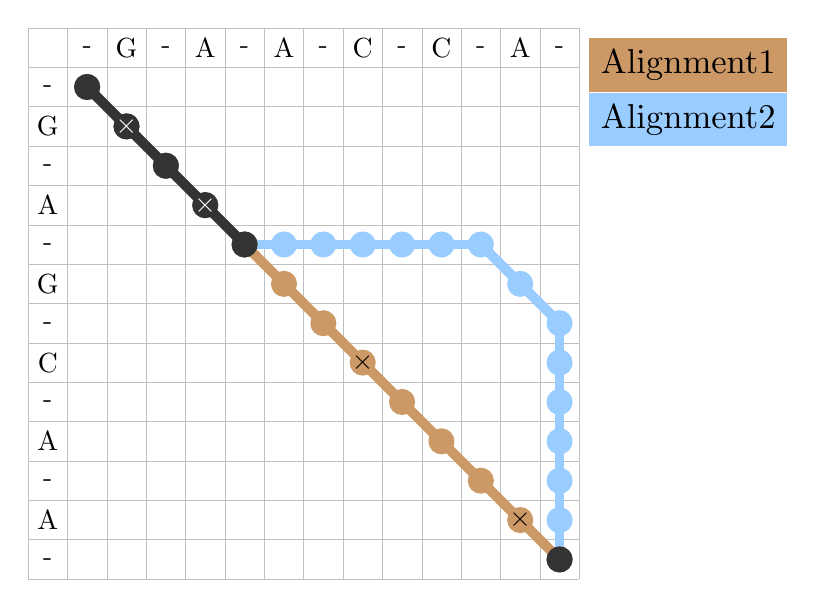
\begin{tikzpicture}[dot/.style={circle, minimum size=2.5mm}, box/.style={rectangle, minimum size = 3.5cm, anchor = north west}]
\draw[very thin, color = gray!50, step = 0.5] (0,0) grid (7, 7);
\node at (0.25,6.25) {-};
\node at (0.25,5.75) {G};
\node at (0.25,5.25) {-};
\node at (0.25,4.75) {A};
\node at (0.25,4.25) {-};
\node at (0.25,3.75) {G};
\node at (0.25,3.25) {-};
\node at (0.25,2.75) {C};
\node at (0.25,2.25) {-};
\node at (0.25,1.75) {A};
\node at (0.25,1.25) {-};
\node at (0.25,0.75) {A};
\node at (0.25,0.25) {-};
\node at (0.75,6.75) {-};
\node at (1.25,6.75) {G};
\node at (1.75,6.75) {-};
\node at (2.25,6.75) {A};
\node at (2.75,6.75) {-};
\node at (3.25,6.75) {A};
\node at (3.75,6.75) {-};
\node at (4.25,6.75) {C};
\node at (4.75,6.75) {-};
\node at (5.25,6.75) {C};
\node at (5.75,6.75) {-};
\node at (6.25,6.75) {A};
\node at (6.75,6.75) {-};
\draw[line width=1.25mm,color2](0.75,6.25)--(1.25,5.75);
\node[circle, fill=color2] at (0.75, 6.25){};
\draw[line width=1.25mm,color2](1.25,5.75)--(1.75,5.25);
\node[circle, fill=color2] at (1.25, 5.75){};
\node[black] at (1.25, 5.75){$\mathlarger{\mathlarger{\bm{\times}}}$};
\draw[line width=1.25mm,color2](1.75,5.25)--(2.25,4.75);
\node[circle, fill=color2] at (1.75, 5.25){};
\draw[line width=1.25mm,color2](2.25,4.75)--(2.75,4.25);
\node[circle, fill=color2] at (2.25, 4.75){};
\node[black] at (2.25, 4.75){$\mathlarger{\mathlarger{\bm{\times}}}$};
\draw[line width=1.25mm,color2](2.75,4.25)--(3.25,4.25);
\node[circle, fill=color2] at (2.75, 4.25){};
\draw[line width=1.25mm,color2](3.25,4.25)--(3.75,4.25);
\node[circle, fill=color2] at (3.25, 4.25){};
\draw[line width=1.25mm,color2](3.75,4.25)--(4.25,4.25);
\node[circle, fill=color2] at (3.75, 4.25){};
\draw[line width=1.25mm,color2](4.25,4.25)--(4.75,4.25);
\node[circle, fill=color2] at (4.25, 4.25){};
\draw[line width=1.25mm,color2](4.75,4.25)--(5.25,4.25);
\node[circle, fill=color2] at (4.75, 4.25){};
\draw[line width=1.25mm,color2](5.25,4.25)--(5.75,4.25);
\node[circle, fill=color2] at (5.25, 4.25){};
\draw[line width=1.25mm,color2](5.75,4.25)--(6.25,3.75);
\node[circle, fill=color2] at (5.75, 4.25){};
\draw[line width=1.25mm,color2](6.25,3.75)--(6.75,3.25);
\node[circle, fill=color2] at (6.25, 3.75){};
\draw[line width=1.25mm,color2](6.75,3.25)--(6.75,2.75);
\node[circle, fill=color2] at (6.75, 3.25){};
\draw[line width=1.25mm,color2](6.75,2.75)--(6.75,2.25);
\node[circle, fill=color2] at (6.75, 2.75){};
\draw[line width=1.25mm,color2](6.75,2.25)--(6.75,1.75);
\node[circle, fill=color2] at (6.75, 2.25){};
\draw[line width=1.25mm,color2](6.75,1.75)--(6.75,1.25);
\node[circle, fill=color2] at (6.75, 1.75){};
\draw[line width=1.25mm,color2](6.75,1.25)--(6.75,0.75);
\node[circle, fill=color2] at (6.75, 1.25){};
\draw[line width=1.25mm,color2](6.75,0.75)--(6.75,0.25);
\node[circle, fill=color2] at (6.75, 0.75){};
\node[circle, fill=color2] at (6.75, 0.25){};
\draw[line width=1.25mm,color1](0.75,6.25)--(1.25,5.75);
\node[circle, fill=color1] at (0.75, 6.25){};
\draw[line width=1.25mm,color1](1.25,5.75)--(1.75,5.25);
\node[circle, fill=color1] at (1.25, 5.75){};
\node[black] at (1.25, 5.75){$\mathlarger{\mathlarger{\bm{\times}}}$};
\draw[line width=1.25mm,color1](1.75,5.25)--(2.25,4.75);
\node[circle, fill=color1] at (1.75, 5.25){};
\draw[line width=1.25mm,color1](2.25,4.75)--(2.75,4.25);
\node[circle, fill=color1] at (2.25, 4.75){};
\node[black] at (2.25, 4.75){$\mathlarger{\mathlarger{\bm{\times}}}$};
\draw[line width=1.25mm,color1](2.75,4.25)--(3.25,3.75);
\node[circle, fill=color1] at (2.75, 4.25){};
\draw[line width=1.25mm,color1](3.25,3.75)--(3.75,3.25);
\node[circle, fill=color1] at (3.25, 3.75){};
\draw[line width=1.25mm,color1](3.75,3.25)--(4.25,2.75);
\node[circle, fill=color1] at (3.75, 3.25){};
\draw[line width=1.25mm,color1](4.25,2.75)--(4.75,2.25);
\node[circle, fill=color1] at (4.25, 2.75){};
\node[black] at (4.25, 2.75){$\mathlarger{\mathlarger{\bm{\times}}}$};
\draw[line width=1.25mm,color1](4.75,2.25)--(5.25,1.75);
\node[circle, fill=color1] at (4.75, 2.25){};
\draw[line width=1.25mm,color1](5.25,1.75)--(5.75,1.25);
\node[circle, fill=color1] at (5.25, 1.75){};
\draw[line width=1.25mm,color1](5.75,1.25)--(6.25,0.75);
\node[circle, fill=color1] at (5.75, 1.25){};
\draw[line width=1.25mm,color1](6.25,0.75)--(6.75,0.25);
\node[circle, fill=color1] at (6.25, 0.75){};
\node[black] at (6.25, 0.75){$\mathlarger{\mathlarger{\bm{\times}}}$};
\node[circle, fill=color1] at (6.75, 0.25){};
\draw[line width=1.25mm,black!80](0.75,6.25)--(1.25,5.75);
\node[circle, fill=black!80] at (0.75, 6.25){};
\draw[line width=1.25mm,black!80](1.25,5.75)--(1.75,5.25);
\node[circle, fill=black!80] at (1.25, 5.75){};
\node[white] at (1.25, 5.75){$\mathlarger{\mathlarger{\bm{\times}}}$};
\draw[line width=1.25mm,black!80](1.75,5.25)--(2.25,4.75);
\node[circle, fill=black!80] at (1.75, 5.25){};
\draw[line width=1.25mm,black!80](2.25,4.75)--(2.75,4.25);
\node[circle, fill=black!80] at (2.25, 4.75){};
\node[white] at (2.25, 4.75){$\mathlarger{\mathlarger{\bm{\times}}}$};
\node[circle, fill=black!80] at (2.75, 4.25){};
\node[circle, fill=black!80] at (6.75, 0.25){};
\matrix [draw, below right, draw=none] at (current bounding box.north east) {
        \node[rectangle, fill=color1, scale=1.25] {Alignment1}; \\
        \node[rectangle, fill=color2, scale=1.25] {Alignment2}; \\
    };
\end{tikzpicture}

\end{multicols}
 \vspace{1mm}
 \caption[Dot plot example]{Example of a visual representation of the region where two pairwise alignments differ. Both sequences are 180 nucleotides long, although only the section where they differ is shown. The figure displays two preceding residues to show complete codons. Alignment 1 is colored in brown and alignment 2 is colored in blue, while matching portions of the alignment are in black. Nodes represent matches, mismatches, and gaps, while edges connect them to form a path. Matches in the alignment are marked with an `X' at the corresponding node.}
 \label{fig:dotplot-example}
\end{figure}

\clearpage

%%%%%%%%%%%%%%%%%%%%%%%%%%%%%%%%%%%%%%%%%%%%%%%%%%%%%%%%%%%%%%%%%%%%%%%%%%%%%%%%
\section{Results}

\subsection{Alignment Accuracy} %%%%%%%%%%%%%%%%%%%%%%%%%%%%%%%%%%%%%%%%%%%%%%%%

\subsubsection{MG94}

The triplet MG94 model consistently outperformed the marginal MG94 models across all datasets (Fig.~\ref{fig:results_tri_mar_mg}). At the lowest branch length of $0.2$, the average alignment error among all three models is similar. However, an evident order emerges, with the triplet-mg model outperforming marginal-mg, which, in turn, achieved a smaller $d_{seq}$ than modal-mg. As the number of expected substitutions increases, the $d_{dseq}$ for the marginal-mg model consistently remains close to that of the triplet model, although the latter outperforms the former across all branch lengths. In contrast, the average alignment error for the modal-mg model diverges further from the other models, spiking when, on average, we expect every site to have undergone a mutation (branch length of 1), with a $d_{seq}$ more than twofold its previous value.

\begin{figure}[!ht]
\centering
\includegraphics[width=\linewidth]{chapter3/figures/results/results_marginal_triplet_mg.pdf}
 \vspace{1mm}
 \caption[Alignment Accuracy of the Triplet and Approximate MG94 Models]{The triplet-mg model generates better alignments across all branch lengths. Results of triplet-mg, marginal-mg, and modal-mg COATi models in aligning 13,758 simulated sequence pairs. Best alignments have the lowest $d_{seq}$, perfect alignments have the same score as the true alignment or a zero $d_{seq}$, and imperfect alignments have a different score than true alignments when at least one model found a perfect alignment.}
 \label{fig:results_tri_mar_mg}
\end{figure}

The number of perfect alignments between the marginal-mg and triplet-mg model remains consistent across all branch lengths. In contrast, the marginal-mg starts producing an equal number of perfect alignments for a branch length of $0.2$, but this number declines as branch lengths increase. A similar trend is observed in the count of imperfect alignments, with the modal-mg model producing more imperfect alignments, particularly spiking at branch lengths of $0.8$ and $1.0$. In this section, the remaining models performed similarly, with the marginal-mg model outperforming the triplet-mg model with branch lengths $0.6$ and $0.8$, with the reverse outcome for branch lengths $0.2$, $0.4$, and $1.0$. Note that the count of perfect and imperfect alignments decreases along the x-axis, as alignments not perfectly retrieved by either method are excluded from the results.

\subsubsection{ECM}

As expected, the triplet-ecm model outperforms the marginal models across all branch lengths in all metrics (Fig.~\ref{fig:results_tri_mar_ecm}). The trend observed in the MG94 results is intensified in the ECM results. The $d_{seq}$ values for the triplet-ecm and marginal-ecm models are comparable to their MG94 counterparts, albeit with a slightly larger difference between them. This pattern is also evident in the number of perfect and imperfect alignments, where the triplet-ecm model significantly outperforms the approximate models. However, the marginal-ecm model provides a better approximation. In contrast, the modal-ecm model underperforms with a $d_{seq}$ two orders of magnitude larger than its MG94 counterpart for a branch length of 1. The model struggles with short branch lengths, and its performance declines as the number of expected substitutions per site increases. I have truncated the $d_{seq}$ values at $0.05$ to ensure a proper display of the results for the triplet-ecm and marginal-ecm. A comprehensive results table can be found in the appendix (Table \ref{table:results-ecm}).

\begin{figure}[!ht]
\centering
\includegraphics[width=\linewidth]{chapter3/figures/results/results_marginal_triplet_ecm.pdf}
 \vspace{1mm}
 \caption[Alignment Accuracy of the Triplet and Approximate ECM Models]{The triplet-ecm model generates better alignments across all branch lengths. Results of triplet-ecm, modal-ecm, and marginal-ecm COATi models in aligning 13,758 simulated sequence pairs. Best alignments have the lowest $d_{seq}$, perfect alignments have the same score as the true alignment or a zero $d_{seq}$, and imperfect alignments have a different score than true alignments when at least one model found a perfect alignment.}
 \label{fig:results_tri_mar_ecm}
\end{figure}

\subsection{Gap Statistics} %%%%%%%%%%%%%%%%%%%%%%%%%%%%%%%%%%%%%%%%%%%%%%%%%%%%%%%%%%%%%%

Gap statistics can provide valuable insights when comparing alignment models across varying evolutionary distances, as they reveal how the likelihood of substitution relative to indel probabilities changes. Notably, for both the MG94 and ECM models, the total number of gaps and their cumulative length remains constant for both the triplet and marginal models as branch lengths increase (Fig.~\ref{fig:results_tri_mar_mg_gaps}). In concordance with the previous metrics, the behavior of the modal model takes a divergent path, especially for modal-ecm. While the modal-mg model shows similar values until branch length reaches $0.6$ and is slightly elevated thereafter, the total number and length of gaps for the modal-ecm model are larger for all branch lengths.

\begin{figure}[!ht]
\centering
\includegraphics[width = 0.75\linewidth]{chapter3/figures/results/results_marginal_triplet_mg_gaps.pdf}
 \vspace{1mm}
 \caption[MG94 Dataset Indel Statistics]{The number and total length of gaps for triplet-mg and marginal-mg models stay constant as branch lengths increase. On the contrary, the modal-mg model adds more and longer gaps as the evolutionary distance between sequences becomes larger.}
 \label{fig:results_tri_mar_mg_gaps}
\end{figure}

\begin{figure}[!ht]
\centering
\includegraphics[width = 0.75\linewidth]{chapter3/figures/results/results_marginal_triplet_ecm_gaps.pdf}
 \vspace{1mm}
 \caption[ECM Dataset Indel Statistics]{The number and total length of gaps for triplet-ecm and marginal-ecm models stay constant as branch lengths increase. On the contrary, the modal-ecm model significantly adds more and longer gaps as the evolutionary distance between sequences becomes larger.}
 \label{fig:results_tri_mar_ecm_gaps}
\end{figure}

\clearpage

\subsection{Marginal Model}

The results from the previous section establish the marginal model as a close approximation to the triplet model. To better understand how marginalization influences the substitution probabilities, I plotted the Kullback-Leibler divergence ($D_{KL}$) between the marginal and the triplet model. This score can be seen as the measure of how one probability distribution, the marginal, differs from a reference probability distribution, the triplet. Figure \ref{fig:kld} is a plot of $D_{KL}$ for the MG94 marginal (top) and ECM marginal (bottom) models with branch length values from 0.1 to 10. The divergence for both marginal models follows a similar trend, with values rising until they reach saturation to then tend towards zero. Marginal-mg is a better approximation to its triplet counterpart than marginal-ecm with smaller values across all branch lengths.
% Sum-mg is a better approximation, with smaller divergence values for all branch lengths. While at the starting branch length of $0.2$ both models have a similar divergence, the values for max-mg increase rapidly. Values for both models increase until they reach saturation, where ultimately their divergence with MG94 decreases.
% Figure \ref{fig:kld}-bottom shows a similar pattern for the ECM case. Sum-ecm also performs best across all branch lengths, with similar values to max-ecm for a branch length of $0.2$. However, both ECM marginal models have a more pronounced curve than their MG94 counterparts, reaching higher divergence values. Additionally, sum-ecm and max-ecm reach saturation and their $D_{KL}$ tends towards zero.

% I analyzed the mutation rates of the triplet model at different branch lengths. The substitution probabilities are plotted in a 61 by 61 matrix, representing codon-to-codon rates, with values ranging from 0 to 1. In this matrix, each column corresponds to the probabilities of a specific codon being replaced by any of the other 61. By definition, shorter branch lengths equate to a small number of expected substitutions per position. Consequently, the majority of the probabilities in the matrix are concentrated along the main diagonal (Fig.~\ref{fig:ptri-02}), indicating substitutions are most likely to retain the same codon.

% Conversely, with longer branch lengths, the distribution of probabilities within each column is not concentrated in one cell and becomes more scattered. Notably, transitions and transversions in the third position of each codon become visible and distinguishable from each other as they begin accumulating probability mass, with transition harnessing a higher probability (Fig.~\ref{fig:ptri-08}). In addition, the increase of first and second-position transition probabilities becomes noticeable.

\begin{figure}[!ht]
    \centering
    \includegraphics[width = 0.9\textwidth]{chapter3/figures/heatmaps/kld_mg.pdf}
    \includegraphics[width = 0.9\textwidth]{chapter3/figures/heatmaps/kld_ecm.pdf}
    \caption[Marginal KL Divergence]{Kullback-Leibler divergence between MG94 (top) ECM (bottom) and their marginal models with branch lengths between 0.2 and 10. Low values represent a small divergence, indicating a better approximation to the triplet model. Marginal MG94 performs best, while the divergence for both models decreases as they reach saturation.}
    \label{fig:kld}
\end{figure}

In addition to the overall measure of divergence, I plotted the $D_{KL}$ matrix between the triplet and marginal model at a branch length of 1 to understand what substitutions drive this score. This 61 by 61 matrix plot represents individual divergence values calculated using $D_{KL}$ (Eq. \ref{eq:KLD}), where blue cells indicate substitution probabilities that are underestimated by the marginal model, while red cells indicate overestimation.
% Figure \ref{fig:kld-max-mg} shows the divergence scores for the max MG94 model. The divergence in this model is driven by a general overestimation along the main diagonal and for first and third-position changes. The most underestimated amino acids are tyrosine and leucine, as shown by a blue predominant section in the top right of the figure, and the most overestimated amino acid is arginine, depicted by a red square along the main diagonal.
Figure \ref{fig:kld-sum-mg} shows the divergence scores for the marginal model. The divergence is driven by a combination of an underestimation of transversions and an overestimation of transitions on the first and third-position mutations.
% Note that the divergence is two orders of magnitude smaller than for the max-mg.
In this case, the most underestimated amino acids are Leucine and Serine, while the most overestimated are tryptophan and tyrosine.

The divergence matrix for the ECM model is plotted following the codon order used in the original ECM publication \citep{kosiol_ECM_2007}, where the order of nucleotides is \{T, C, A, G\}, and first position changes precede second position ones (Fig. \ref{fig:kld-sum-ecm}).
% The divergence for the max-ecm model is driven by a general overestimation of substitution probabilities, especially along the main diagonal. A blue section on the top right corner portrays an underestimation zone, with amino acids arginine and serine being the most underestimated by this model.
The $D_{KL}$ divergence for the marginal-ecm model is driven by a general overestimation of substitution probabilities, especially along the main diagonal (indicating no change). In addition, we observe an underestimation of the arginine and serine amino acids (top left blue section). The most overestimated amino acids include histidine, although the difference is small. Notably, the divergence values for the marginal ECM model are much higher than for the MG94 counterpart.

% \begin{figure}[!ht]
%     \centering
%     % \includegraphics[width = 0.8\textwidth]{chapter3/figures/heatmaps/tri-max-mg-0.2.pdf}
%     \includegraphics[width = \textwidth]{chapter3/figures/heatmaps/tri-max-mg-1.pdf}
%     \caption[Max-mg Kullback-Leibler Divergence Matrix]{Kullback-Leibler divergence matrix for the max MG94 model with a branch length of $1.0$. Values closer to zero indicate a smaller divergence, representing a better approximation to the triplet model. Positive values, indicated by a blue gradient, mark substitution probabilities where max underestimates the triplet model. In turn, negative values, indicated by a red gradient, represent substitution probabilities where max overestimates the triplet model.}
%     \label{fig:kld-max-mg}
% \end{figure}

\begin{figure}[!ht]
    \centering
    % \includegraphics[width = 0.8\textwidth]{chapter3/figures/heatmaps/tri-sum-mg-0.2.pdf}
    \includegraphics[width = \textwidth]{chapter3/figures/heatmaps/tri-sum-mg-1.pdf}
    \caption[Marginal-mg Kullback-Leibler Divergence Matrix]{Kullback-Leibler divergence matrix for the marginal MG94 model with a branch length of $1.0$. Values closer to zero indicate a smaller divergence, representing a better approximation to the triplet model. Positive values, indicated by a blue gradient, mark substitution probabilities where the marginal model underestimates the triplet model. In turn, negative values, indicated by a red gradient, represent substitution probabilities where marginal overestimates the triplet model.}
    \label{fig:kld-sum-mg}
\end{figure}

% In addition to the overall measure of divergence, I analyzed the $D_{KL}$ matrix to understand what substitutions drive this score. Figure \ref{fig:kld-max-mg} shows the divergence scores for the max MG94 model at branch length $1.0$. The divergence in this model is driven by a combination of underestimating and overestimating the triplet along the main diagonal. Tyr is the most overestimated amino acid, while Arg is the most underestimated. For the sum MG94 model, figure \ref{fig:kld-sum-mg} shows the divergence with MG94 at a branch length of $1.0$. In this case, third and second-position transitions drive the divergence with the triplet model. Asn is the most overestimated amino acid, while Trp is the most underestimated.

% \begin{figure}[!ht]
%     \centering
%     % \includegraphics[width = 0.8\textwidth]{chapter3/figures/heatmaps/tri-max-mg-0.2.pdf}
%     \includegraphics[width = \textwidth]{chapter3/figures/heatmaps/tri-max-ecm-1.pdf}
%     \caption[Max-ecm Kullback-Leibler Divergence Matrix]{Kullback-Leibler divergence matrix for the max ECM model with a branch length of $1.0$. Values closer to zero indicate a smaller divergence, representing a better approximation to the triplet model. Positive values, indicated by a blue gradient, mark substitution probabilities where max underestimates the triplet model. In turn, negative values, indicated by a red gradient, represent substitution probabilities where max overestimates the triplet model.}
%     \label{fig:kld-max-ecm}
% \end{figure}

\begin{figure}[!ht]
    \centering
    % \includegraphics[width = 0.8\textwidth]{chapter3/figures/heatmaps/tri-sum-mg-0.2.pdf}
    \includegraphics[width = \textwidth]{chapter3/figures/heatmaps/tri-sum-ecm-1.pdf}
    \caption[Marginal-ecm Kullback-Leibler Divergence Matrix]{Kullback-Leibler divergence matrix for the marginal ECM model with a branch length of $1.0$. Values closer to zero indicate a smaller divergence, representing a better approximation to the triplet model. Positive values, indicated by a blue gradient, mark substitution probabilities where the marginal model underestimates the triplet model. In turn, negative values, indicated by a red gradient, represent substitution probabilities where marginal overestimates the triplet model.}
    \label{fig:kld-sum-ecm}
\end{figure}

\clearpage

\subsection{Visual Comparison of Triplet and Marginal Model} %%%%%%%%%%%%%%%%%%%%%

The previous metrics have demonstrated that the triplet and marginal models exhibit a strong agreement in their results, thereby validating the latter as a suitable approximation of the former. However, these metrics have fallen short in identifying any subtle distinctions between the models, if they exist. Pursuing these differences, I inspected the alignment sections where the two models diverge using dot plots. Upon visual comparison of the most distinct triplet and marginal alignments across sequence lengths spanning from a few hundred to a maximum of three thousand nucleotides and encompassing all branch lengths (0.2, 0.4, 0.6, 0.8, and 1.0), one predominant pattern emerges (examples in Fig.~\ref{fig:dotplots}). The most notable distinction between the triplet and marginal models lies in the former model displaying a preference for substitutions, irrespective of the number of matches, whereas the latter model favors indels, often with a higher number of matches (left column in Figure \ref{fig:dotplots}).
 
\begin{figure}[!ht]
 \centering
 % \setlength{\columnsep}{-4cm}
 \begin{multicols}{2}
% \vspace*{2.5em}
% \hspace{-5cm}
\scalebox{0.52}{\input{chapter3/figures/dotplots/0.8-ENSG00000124383.fasta1}}
\vspace{0.5em}

\scalebox{0.52}{% Created by tikzDevice version 0.12.5 on 2023-10-05 23:41:36
% !TEX encoding = UTF-8 Unicode
\definecolor{triplet}{HTML}{E69F00}
\definecolor{mar-sum}{HTML}{009E73}
\definecolor{mar-max}{HTML}{CC79A7}
\definecolor{color1}{HTML}{CC9966}
\definecolor{color2}{HTML}{99CCFF}
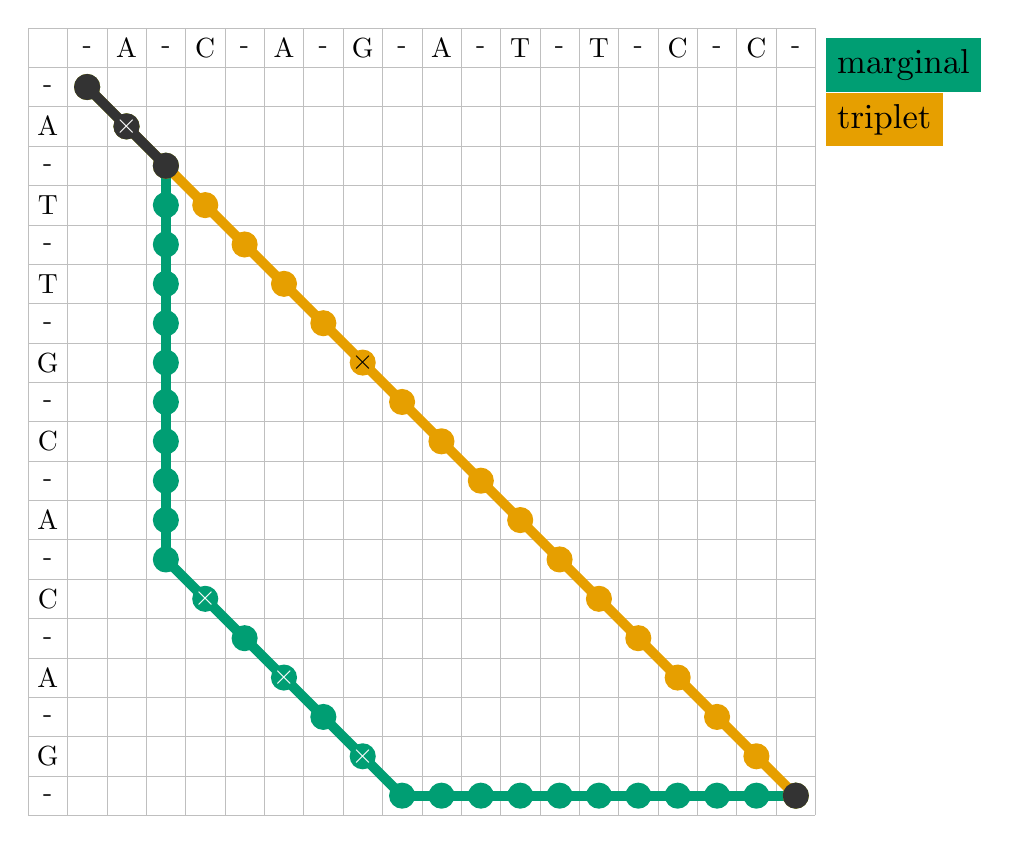
\begin{tikzpicture}[dot/.style={circle, minimum size=2.5mm}, box/.style={rectangle, minimum size = 3.5cm, anchor = north west}]
\draw[very thin, color = gray!50, step = 0.5] (0,0) grid (10, 10);
\node at (0.25,9.25) {-};
\node at (0.25,8.75) {A};
\node at (0.25,8.25) {-};
\node at (0.25,7.75) {T};
\node at (0.25,7.25) {-};
\node at (0.25,6.75) {T};
\node at (0.25,6.25) {-};
\node at (0.25,5.75) {G};
\node at (0.25,5.25) {-};
\node at (0.25,4.75) {C};
\node at (0.25,4.25) {-};
\node at (0.25,3.75) {A};
\node at (0.25,3.25) {-};
\node at (0.25,2.75) {C};
\node at (0.25,2.25) {-};
\node at (0.25,1.75) {A};
\node at (0.25,1.25) {-};
\node at (0.25,0.75) {G};
\node at (0.25,0.25) {-};
\node at (0.75,9.75) {-};
\node at (1.25,9.75) {A};
\node at (1.75,9.75) {-};
\node at (2.25,9.75) {C};
\node at (2.75,9.75) {-};
\node at (3.25,9.75) {A};
\node at (3.75,9.75) {-};
\node at (4.25,9.75) {G};
\node at (4.75,9.75) {-};
\node at (5.25,9.75) {A};
\node at (5.75,9.75) {-};
\node at (6.25,9.75) {T};
\node at (6.75,9.75) {-};
\node at (7.25,9.75) {T};
\node at (7.75,9.75) {-};
\node at (8.25,9.75) {C};
\node at (8.75,9.75) {-};
\node at (9.25,9.75) {C};
\node at (9.75,9.75) {-};
\draw[line width=1.25mm,mar-sum](0.75,9.25)--(1.25,8.75);
\node[circle, fill=mar-sum] at (0.75, 9.25){};
\draw[line width=1.25mm,mar-sum](1.25,8.75)--(1.75,8.25);
\node[circle, fill=mar-sum] at (1.25, 8.75){};
\node[white] at (1.25, 8.75){$\mathlarger{\mathlarger{\bm{\times}}}$};
\draw[line width=1.25mm,mar-sum](1.75,8.25)--(1.75,7.75);
\node[circle, fill=mar-sum] at (1.75, 8.25){};
\draw[line width=1.25mm,mar-sum](1.75,7.75)--(1.75,7.25);
\node[circle, fill=mar-sum] at (1.75, 7.75){};
\draw[line width=1.25mm,mar-sum](1.75,7.25)--(1.75,6.75);
\node[circle, fill=mar-sum] at (1.75, 7.25){};
\draw[line width=1.25mm,mar-sum](1.75,6.75)--(1.75,6.25);
\node[circle, fill=mar-sum] at (1.75, 6.75){};
\draw[line width=1.25mm,mar-sum](1.75,6.25)--(1.75,5.75);
\node[circle, fill=mar-sum] at (1.75, 6.25){};
\draw[line width=1.25mm,mar-sum](1.75,5.75)--(1.75,5.25);
\node[circle, fill=mar-sum] at (1.75, 5.75){};
\draw[line width=1.25mm,mar-sum](1.75,5.25)--(1.75,4.75);
\node[circle, fill=mar-sum] at (1.75, 5.25){};
\draw[line width=1.25mm,mar-sum](1.75,4.75)--(1.75,4.25);
\node[circle, fill=mar-sum] at (1.75, 4.75){};
\draw[line width=1.25mm,mar-sum](1.75,4.25)--(1.75,3.75);
\node[circle, fill=mar-sum] at (1.75, 4.25){};
\draw[line width=1.25mm,mar-sum](1.75,3.75)--(1.75,3.25);
\node[circle, fill=mar-sum] at (1.75, 3.75){};
\draw[line width=1.25mm,mar-sum](1.75,3.25)--(2.25,2.75);
\node[circle, fill=mar-sum] at (1.75, 3.25){};
\draw[line width=1.25mm,mar-sum](2.25,2.75)--(2.75,2.25);
\node[circle, fill=mar-sum] at (2.25, 2.75){};
\node[white] at (2.25, 2.75){$\mathlarger{\mathlarger{\bm{\times}}}$};
\draw[line width=1.25mm,mar-sum](2.75,2.25)--(3.25,1.75);
\node[circle, fill=mar-sum] at (2.75, 2.25){};
\draw[line width=1.25mm,mar-sum](3.25,1.75)--(3.75,1.25);
\node[circle, fill=mar-sum] at (3.25, 1.75){};
\node[white] at (3.25, 1.75){$\mathlarger{\mathlarger{\bm{\times}}}$};
\draw[line width=1.25mm,mar-sum](3.75,1.25)--(4.25,0.75);
\node[circle, fill=mar-sum] at (3.75, 1.25){};
\draw[line width=1.25mm,mar-sum](4.25,0.75)--(4.75,0.25);
\node[circle, fill=mar-sum] at (4.25, 0.75){};
\node[white] at (4.25, 0.75){$\mathlarger{\mathlarger{\bm{\times}}}$};
\draw[line width=1.25mm,mar-sum](4.75,0.25)--(5.25,0.25);
\node[circle, fill=mar-sum] at (4.75, 0.25){};
\draw[line width=1.25mm,mar-sum](5.25,0.25)--(5.75,0.25);
\node[circle, fill=mar-sum] at (5.25, 0.25){};
\draw[line width=1.25mm,mar-sum](5.75,0.25)--(6.25,0.25);
\node[circle, fill=mar-sum] at (5.75, 0.25){};
\draw[line width=1.25mm,mar-sum](6.25,0.25)--(6.75,0.25);
\node[circle, fill=mar-sum] at (6.25, 0.25){};
\draw[line width=1.25mm,mar-sum](6.75,0.25)--(7.25,0.25);
\node[circle, fill=mar-sum] at (6.75, 0.25){};
\draw[line width=1.25mm,mar-sum](7.25,0.25)--(7.75,0.25);
\node[circle, fill=mar-sum] at (7.25, 0.25){};
\draw[line width=1.25mm,mar-sum](7.75,0.25)--(8.25,0.25);
\node[circle, fill=mar-sum] at (7.75, 0.25){};
\draw[line width=1.25mm,mar-sum](8.25,0.25)--(8.75,0.25);
\node[circle, fill=mar-sum] at (8.25, 0.25){};
\draw[line width=1.25mm,mar-sum](8.75,0.25)--(9.25,0.25);
\node[circle, fill=mar-sum] at (8.75, 0.25){};
\draw[line width=1.25mm,mar-sum](9.25,0.25)--(9.75,0.25);
\node[circle, fill=mar-sum] at (9.25, 0.25){};
\node[circle, fill=mar-sum] at (9.75, 0.25){};
\draw[line width=1.25mm,triplet](0.75,9.25)--(1.25,8.75);
\node[circle, fill=triplet] at (0.75, 9.25){};
\draw[line width=1.25mm,triplet](1.25,8.75)--(1.75,8.25);
\node[circle, fill=triplet] at (1.25, 8.75){};
\node[black] at (1.25, 8.75){$\mathlarger{\mathlarger{\bm{\times}}}$};
\draw[line width=1.25mm,triplet](1.75,8.25)--(2.25,7.75);
\node[circle, fill=triplet] at (1.75, 8.25){};
\draw[line width=1.25mm,triplet](2.25,7.75)--(2.75,7.25);
\node[circle, fill=triplet] at (2.25, 7.75){};
\draw[line width=1.25mm,triplet](2.75,7.25)--(3.25,6.75);
\node[circle, fill=triplet] at (2.75, 7.25){};
\draw[line width=1.25mm,triplet](3.25,6.75)--(3.75,6.25);
\node[circle, fill=triplet] at (3.25, 6.75){};
\draw[line width=1.25mm,triplet](3.75,6.25)--(4.25,5.75);
\node[circle, fill=triplet] at (3.75, 6.25){};
\draw[line width=1.25mm,triplet](4.25,5.75)--(4.75,5.25);
\node[circle, fill=triplet] at (4.25, 5.75){};
\node[black] at (4.25, 5.75){$\mathlarger{\mathlarger{\bm{\times}}}$};
\draw[line width=1.25mm,triplet](4.75,5.25)--(5.25,4.75);
\node[circle, fill=triplet] at (4.75, 5.25){};
\draw[line width=1.25mm,triplet](5.25,4.75)--(5.75,4.25);
\node[circle, fill=triplet] at (5.25, 4.75){};
\draw[line width=1.25mm,triplet](5.75,4.25)--(6.25,3.75);
\node[circle, fill=triplet] at (5.75, 4.25){};
\draw[line width=1.25mm,triplet](6.25,3.75)--(6.75,3.25);
\node[circle, fill=triplet] at (6.25, 3.75){};
\draw[line width=1.25mm,triplet](6.75,3.25)--(7.25,2.75);
\node[circle, fill=triplet] at (6.75, 3.25){};
\draw[line width=1.25mm,triplet](7.25,2.75)--(7.75,2.25);
\node[circle, fill=triplet] at (7.25, 2.75){};
\draw[line width=1.25mm,triplet](7.75,2.25)--(8.25,1.75);
\node[circle, fill=triplet] at (7.75, 2.25){};
\draw[line width=1.25mm,triplet](8.25,1.75)--(8.75,1.25);
\node[circle, fill=triplet] at (8.25, 1.75){};
\draw[line width=1.25mm,triplet](8.75,1.25)--(9.25,0.75);
\node[circle, fill=triplet] at (8.75, 1.25){};
\draw[line width=1.25mm,triplet](9.25,0.75)--(9.75,0.25);
\node[circle, fill=triplet] at (9.25, 0.75){};
\node[circle, fill=triplet] at (9.75, 0.25){};
\draw[line width=1.25mm,black!80](0.75,9.25)--(1.25,8.75);
\node[circle, fill=black!80] at (0.75, 9.25){};
\draw[line width=1.25mm,black!80](1.25,8.75)--(1.75,8.25);
\node[circle, fill=black!80] at (1.25, 8.75){};
\node[white] at (1.25, 8.75){$\mathlarger{\mathlarger{\bm{\times}}}$};
\node[circle, fill=black!80] at (1.75, 8.25){};
\node[circle, fill=black!80] at (9.75, 0.25){};
\matrix [draw, below right, draw=none] at (current bounding box.north east) {
        \node[rectangle, fill=mar-sum, scale=1.25] {marginal}; \\
        \node[rectangle, fill=triplet, scale=1.25] {triplet}; \\
    };
\end{tikzpicture}
}
\vspace{0.5em}

\scalebox{0.42}{\input{chapter3/figures/dotplots/0.2-ENSG00000082074.fasta1}}
\columnbreak

\scalebox{0.40}{\input{chapter3/figures/dotplots/0.2-ENSG00000166669.fasta-ecm1}}
\vspace{0.5em}

\scalebox{0.40}{\input{chapter3/figures/dotplots/0.2-ENSG00000166669.fasta-ecm3}}
\vspace{0.5em}

\scalebox{0.34}{% Created by tikzDevice version 0.12.5 on 2023-10-05 23:41:38
% !TEX encoding = UTF-8 Unicode
\definecolor{triplet}{HTML}{E69F00}
\definecolor{mar-sum}{HTML}{009E73}
\definecolor{mar-max}{HTML}{CC79A7}
\definecolor{color1}{HTML}{CC9966}
\definecolor{color2}{HTML}{99CCFF}
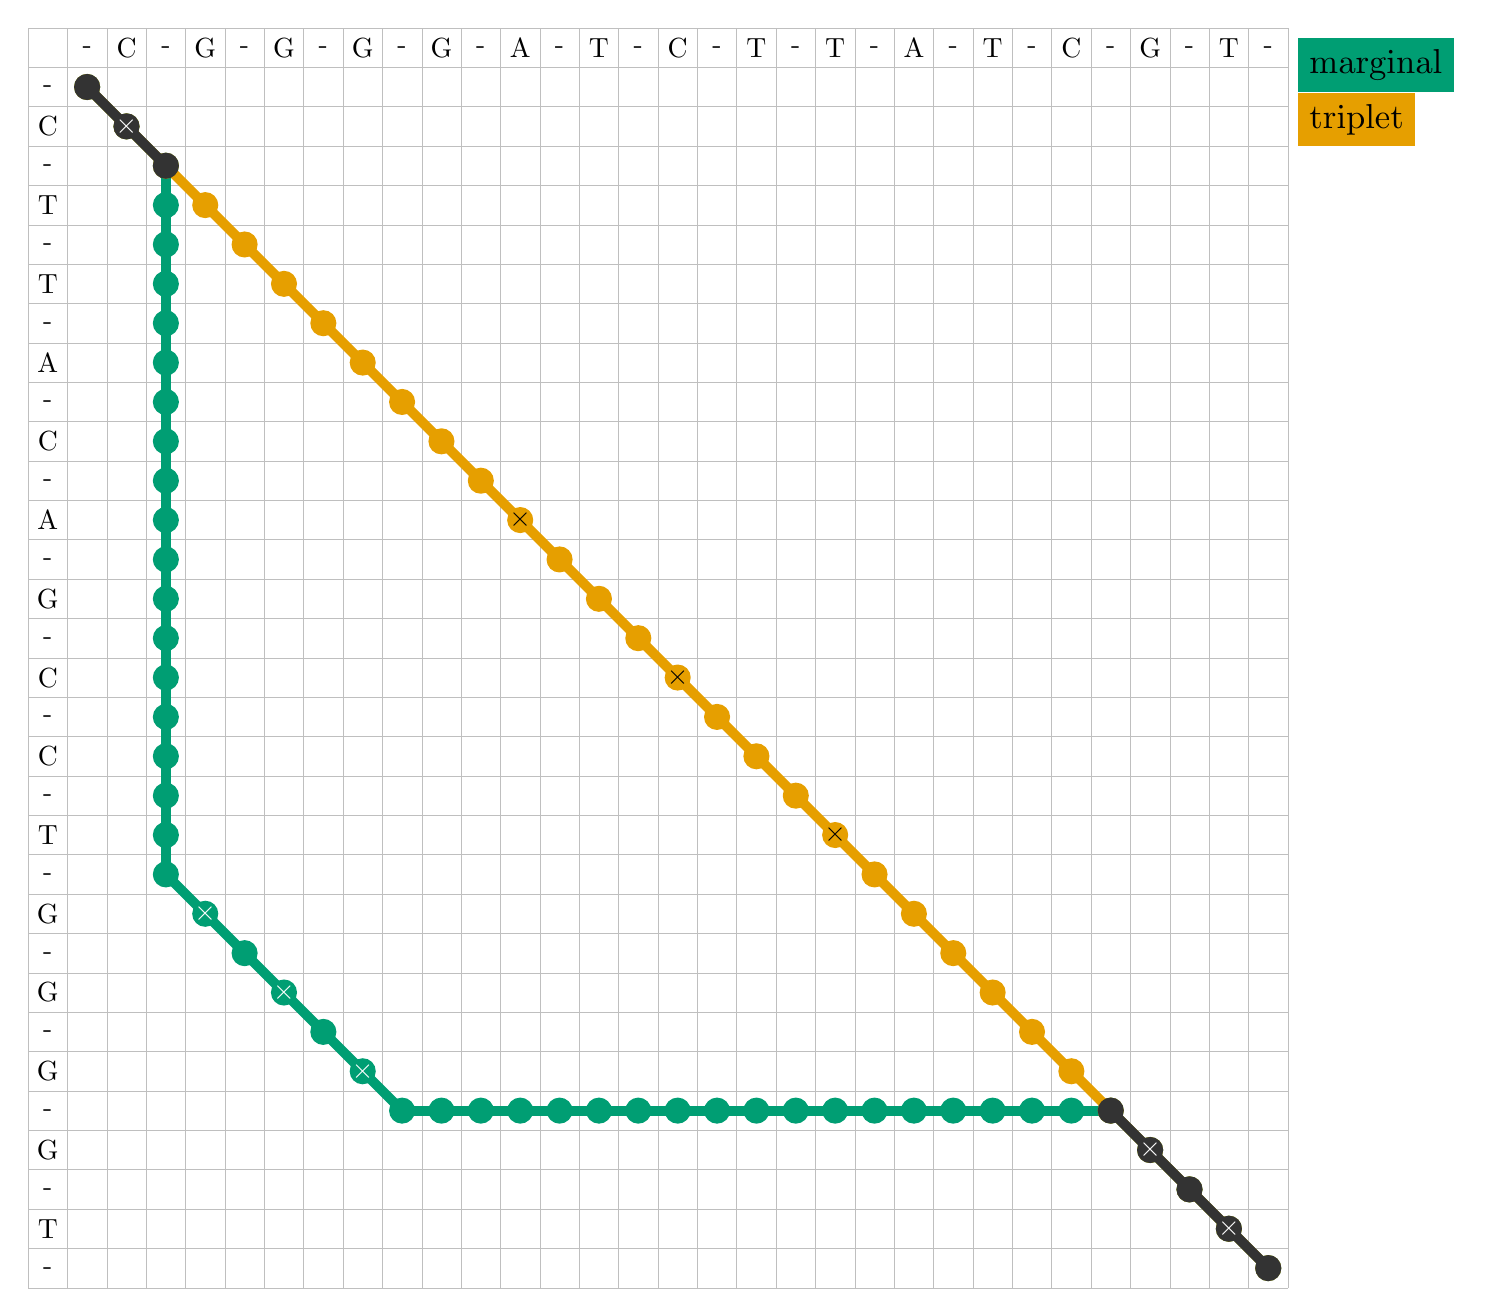
\begin{tikzpicture}[dot/.style={circle, minimum size=2.5mm}, box/.style={rectangle, minimum size = 3.5cm, anchor = north west}]
\draw[very thin, color = gray!50, step = 0.5] (0,0) grid (16, 16);
\node at (0.25,15.25) {-};
\node at (0.25,14.75) {C};
\node at (0.25,14.25) {-};
\node at (0.25,13.75) {T};
\node at (0.25,13.25) {-};
\node at (0.25,12.75) {T};
\node at (0.25,12.25) {-};
\node at (0.25,11.75) {A};
\node at (0.25,11.25) {-};
\node at (0.25,10.75) {C};
\node at (0.25,10.25) {-};
\node at (0.25,9.75) {A};
\node at (0.25,9.25) {-};
\node at (0.25,8.75) {G};
\node at (0.25,8.25) {-};
\node at (0.25,7.75) {C};
\node at (0.25,7.25) {-};
\node at (0.25,6.75) {C};
\node at (0.25,6.25) {-};
\node at (0.25,5.75) {T};
\node at (0.25,5.25) {-};
\node at (0.25,4.75) {G};
\node at (0.25,4.25) {-};
\node at (0.25,3.75) {G};
\node at (0.25,3.25) {-};
\node at (0.25,2.75) {G};
\node at (0.25,2.25) {-};
\node at (0.25,1.75) {G};
\node at (0.25,1.25) {-};
\node at (0.25,0.75) {T};
\node at (0.25,0.25) {-};
\node at (0.75,15.75) {-};
\node at (1.25,15.75) {C};
\node at (1.75,15.75) {-};
\node at (2.25,15.75) {G};
\node at (2.75,15.75) {-};
\node at (3.25,15.75) {G};
\node at (3.75,15.75) {-};
\node at (4.25,15.75) {G};
\node at (4.75,15.75) {-};
\node at (5.25,15.75) {G};
\node at (5.75,15.75) {-};
\node at (6.25,15.75) {A};
\node at (6.75,15.75) {-};
\node at (7.25,15.75) {T};
\node at (7.75,15.75) {-};
\node at (8.25,15.75) {C};
\node at (8.75,15.75) {-};
\node at (9.25,15.75) {T};
\node at (9.75,15.75) {-};
\node at (10.25,15.75) {T};
\node at (10.75,15.75) {-};
\node at (11.25,15.75) {A};
\node at (11.75,15.75) {-};
\node at (12.25,15.75) {T};
\node at (12.75,15.75) {-};
\node at (13.25,15.75) {C};
\node at (13.75,15.75) {-};
\node at (14.25,15.75) {G};
\node at (14.75,15.75) {-};
\node at (15.25,15.75) {T};
\node at (15.75,15.75) {-};
\draw[line width=1.25mm,mar-sum](0.75,15.25)--(1.25,14.75);
\node[circle, fill=mar-sum] at (0.75, 15.25){};
\draw[line width=1.25mm,mar-sum](1.25,14.75)--(1.75,14.25);
\node[circle, fill=mar-sum] at (1.25, 14.75){};
\node[white] at (1.25, 14.75){$\mathlarger{\mathlarger{\bm{\times}}}$};
\draw[line width=1.25mm,mar-sum](1.75,14.25)--(1.75,13.75);
\node[circle, fill=mar-sum] at (1.75, 14.25){};
\draw[line width=1.25mm,mar-sum](1.75,13.75)--(1.75,13.25);
\node[circle, fill=mar-sum] at (1.75, 13.75){};
\draw[line width=1.25mm,mar-sum](1.75,13.25)--(1.75,12.75);
\node[circle, fill=mar-sum] at (1.75, 13.25){};
\draw[line width=1.25mm,mar-sum](1.75,12.75)--(1.75,12.25);
\node[circle, fill=mar-sum] at (1.75, 12.75){};
\draw[line width=1.25mm,mar-sum](1.75,12.25)--(1.75,11.75);
\node[circle, fill=mar-sum] at (1.75, 12.25){};
\draw[line width=1.25mm,mar-sum](1.75,11.75)--(1.75,11.25);
\node[circle, fill=mar-sum] at (1.75, 11.75){};
\draw[line width=1.25mm,mar-sum](1.75,11.25)--(1.75,10.75);
\node[circle, fill=mar-sum] at (1.75, 11.25){};
\draw[line width=1.25mm,mar-sum](1.75,10.75)--(1.75,10.25);
\node[circle, fill=mar-sum] at (1.75, 10.75){};
\draw[line width=1.25mm,mar-sum](1.75,10.25)--(1.75,9.75);
\node[circle, fill=mar-sum] at (1.75, 10.25){};
\draw[line width=1.25mm,mar-sum](1.75,9.75)--(1.75,9.25);
\node[circle, fill=mar-sum] at (1.75, 9.75){};
\draw[line width=1.25mm,mar-sum](1.75,9.25)--(1.75,8.75);
\node[circle, fill=mar-sum] at (1.75, 9.25){};
\draw[line width=1.25mm,mar-sum](1.75,8.75)--(1.75,8.25);
\node[circle, fill=mar-sum] at (1.75, 8.75){};
\draw[line width=1.25mm,mar-sum](1.75,8.25)--(1.75,7.75);
\node[circle, fill=mar-sum] at (1.75, 8.25){};
\draw[line width=1.25mm,mar-sum](1.75,7.75)--(1.75,7.25);
\node[circle, fill=mar-sum] at (1.75, 7.75){};
\draw[line width=1.25mm,mar-sum](1.75,7.25)--(1.75,6.75);
\node[circle, fill=mar-sum] at (1.75, 7.25){};
\draw[line width=1.25mm,mar-sum](1.75,6.75)--(1.75,6.25);
\node[circle, fill=mar-sum] at (1.75, 6.75){};
\draw[line width=1.25mm,mar-sum](1.75,6.25)--(1.75,5.75);
\node[circle, fill=mar-sum] at (1.75, 6.25){};
\draw[line width=1.25mm,mar-sum](1.75,5.75)--(1.75,5.25);
\node[circle, fill=mar-sum] at (1.75, 5.75){};
\draw[line width=1.25mm,mar-sum](1.75,5.25)--(2.25,4.75);
\node[circle, fill=mar-sum] at (1.75, 5.25){};
\draw[line width=1.25mm,mar-sum](2.25,4.75)--(2.75,4.25);
\node[circle, fill=mar-sum] at (2.25, 4.75){};
\node[white] at (2.25, 4.75){$\mathlarger{\mathlarger{\bm{\times}}}$};
\draw[line width=1.25mm,mar-sum](2.75,4.25)--(3.25,3.75);
\node[circle, fill=mar-sum] at (2.75, 4.25){};
\draw[line width=1.25mm,mar-sum](3.25,3.75)--(3.75,3.25);
\node[circle, fill=mar-sum] at (3.25, 3.75){};
\node[white] at (3.25, 3.75){$\mathlarger{\mathlarger{\bm{\times}}}$};
\draw[line width=1.25mm,mar-sum](3.75,3.25)--(4.25,2.75);
\node[circle, fill=mar-sum] at (3.75, 3.25){};
\draw[line width=1.25mm,mar-sum](4.25,2.75)--(4.75,2.25);
\node[circle, fill=mar-sum] at (4.25, 2.75){};
\node[white] at (4.25, 2.75){$\mathlarger{\mathlarger{\bm{\times}}}$};
\draw[line width=1.25mm,mar-sum](4.75,2.25)--(5.25,2.25);
\node[circle, fill=mar-sum] at (4.75, 2.25){};
\draw[line width=1.25mm,mar-sum](5.25,2.25)--(5.75,2.25);
\node[circle, fill=mar-sum] at (5.25, 2.25){};
\draw[line width=1.25mm,mar-sum](5.75,2.25)--(6.25,2.25);
\node[circle, fill=mar-sum] at (5.75, 2.25){};
\draw[line width=1.25mm,mar-sum](6.25,2.25)--(6.75,2.25);
\node[circle, fill=mar-sum] at (6.25, 2.25){};
\draw[line width=1.25mm,mar-sum](6.75,2.25)--(7.25,2.25);
\node[circle, fill=mar-sum] at (6.75, 2.25){};
\draw[line width=1.25mm,mar-sum](7.25,2.25)--(7.75,2.25);
\node[circle, fill=mar-sum] at (7.25, 2.25){};
\draw[line width=1.25mm,mar-sum](7.75,2.25)--(8.25,2.25);
\node[circle, fill=mar-sum] at (7.75, 2.25){};
\draw[line width=1.25mm,mar-sum](8.25,2.25)--(8.75,2.25);
\node[circle, fill=mar-sum] at (8.25, 2.25){};
\draw[line width=1.25mm,mar-sum](8.75,2.25)--(9.25,2.25);
\node[circle, fill=mar-sum] at (8.75, 2.25){};
\draw[line width=1.25mm,mar-sum](9.25,2.25)--(9.75,2.25);
\node[circle, fill=mar-sum] at (9.25, 2.25){};
\draw[line width=1.25mm,mar-sum](9.75,2.25)--(10.25,2.25);
\node[circle, fill=mar-sum] at (9.75, 2.25){};
\draw[line width=1.25mm,mar-sum](10.25,2.25)--(10.75,2.25);
\node[circle, fill=mar-sum] at (10.25, 2.25){};
\draw[line width=1.25mm,mar-sum](10.75,2.25)--(11.25,2.25);
\node[circle, fill=mar-sum] at (10.75, 2.25){};
\draw[line width=1.25mm,mar-sum](11.25,2.25)--(11.75,2.25);
\node[circle, fill=mar-sum] at (11.25, 2.25){};
\draw[line width=1.25mm,mar-sum](11.75,2.25)--(12.25,2.25);
\node[circle, fill=mar-sum] at (11.75, 2.25){};
\draw[line width=1.25mm,mar-sum](12.25,2.25)--(12.75,2.25);
\node[circle, fill=mar-sum] at (12.25, 2.25){};
\draw[line width=1.25mm,mar-sum](12.75,2.25)--(13.25,2.25);
\node[circle, fill=mar-sum] at (12.75, 2.25){};
\draw[line width=1.25mm,mar-sum](13.25,2.25)--(13.75,2.25);
\node[circle, fill=mar-sum] at (13.25, 2.25){};
\draw[line width=1.25mm,mar-sum](13.75,2.25)--(14.25,1.75);
\node[circle, fill=mar-sum] at (13.75, 2.25){};
\draw[line width=1.25mm,mar-sum](14.25,1.75)--(14.75,1.25);
\node[circle, fill=mar-sum] at (14.25, 1.75){};
\node[white] at (14.25, 1.75){$\mathlarger{\mathlarger{\bm{\times}}}$};
\draw[line width=1.25mm,mar-sum](14.75,1.25)--(15.25,0.75);
\node[circle, fill=mar-sum] at (14.75, 1.25){};
\draw[line width=1.25mm,mar-sum](15.25,0.75)--(15.75,0.25);
\node[circle, fill=mar-sum] at (15.25, 0.75){};
\node[white] at (15.25, 0.75){$\mathlarger{\mathlarger{\bm{\times}}}$};
\node[circle, fill=mar-sum] at (15.75, 0.25){};
\draw[line width=1.25mm,triplet](0.75,15.25)--(1.25,14.75);
\node[circle, fill=triplet] at (0.75, 15.25){};
\draw[line width=1.25mm,triplet](1.25,14.75)--(1.75,14.25);
\node[circle, fill=triplet] at (1.25, 14.75){};
\node[black] at (1.25, 14.75){$\mathlarger{\mathlarger{\bm{\times}}}$};
\draw[line width=1.25mm,triplet](1.75,14.25)--(2.25,13.75);
\node[circle, fill=triplet] at (1.75, 14.25){};
\draw[line width=1.25mm,triplet](2.25,13.75)--(2.75,13.25);
\node[circle, fill=triplet] at (2.25, 13.75){};
\draw[line width=1.25mm,triplet](2.75,13.25)--(3.25,12.75);
\node[circle, fill=triplet] at (2.75, 13.25){};
\draw[line width=1.25mm,triplet](3.25,12.75)--(3.75,12.25);
\node[circle, fill=triplet] at (3.25, 12.75){};
\draw[line width=1.25mm,triplet](3.75,12.25)--(4.25,11.75);
\node[circle, fill=triplet] at (3.75, 12.25){};
\draw[line width=1.25mm,triplet](4.25,11.75)--(4.75,11.25);
\node[circle, fill=triplet] at (4.25, 11.75){};
\draw[line width=1.25mm,triplet](4.75,11.25)--(5.25,10.75);
\node[circle, fill=triplet] at (4.75, 11.25){};
\draw[line width=1.25mm,triplet](5.25,10.75)--(5.75,10.25);
\node[circle, fill=triplet] at (5.25, 10.75){};
\draw[line width=1.25mm,triplet](5.75,10.25)--(6.25,9.75);
\node[circle, fill=triplet] at (5.75, 10.25){};
\draw[line width=1.25mm,triplet](6.25,9.75)--(6.75,9.25);
\node[circle, fill=triplet] at (6.25, 9.75){};
\node[black] at (6.25, 9.75){$\mathlarger{\mathlarger{\bm{\times}}}$};
\draw[line width=1.25mm,triplet](6.75,9.25)--(7.25,8.75);
\node[circle, fill=triplet] at (6.75, 9.25){};
\draw[line width=1.25mm,triplet](7.25,8.75)--(7.75,8.25);
\node[circle, fill=triplet] at (7.25, 8.75){};
\draw[line width=1.25mm,triplet](7.75,8.25)--(8.25,7.75);
\node[circle, fill=triplet] at (7.75, 8.25){};
\draw[line width=1.25mm,triplet](8.25,7.75)--(8.75,7.25);
\node[circle, fill=triplet] at (8.25, 7.75){};
\node[black] at (8.25, 7.75){$\mathlarger{\mathlarger{\bm{\times}}}$};
\draw[line width=1.25mm,triplet](8.75,7.25)--(9.25,6.75);
\node[circle, fill=triplet] at (8.75, 7.25){};
\draw[line width=1.25mm,triplet](9.25,6.75)--(9.75,6.25);
\node[circle, fill=triplet] at (9.25, 6.75){};
\draw[line width=1.25mm,triplet](9.75,6.25)--(10.25,5.75);
\node[circle, fill=triplet] at (9.75, 6.25){};
\draw[line width=1.25mm,triplet](10.25,5.75)--(10.75,5.25);
\node[circle, fill=triplet] at (10.25, 5.75){};
\node[black] at (10.25, 5.75){$\mathlarger{\mathlarger{\bm{\times}}}$};
\draw[line width=1.25mm,triplet](10.75,5.25)--(11.25,4.75);
\node[circle, fill=triplet] at (10.75, 5.25){};
\draw[line width=1.25mm,triplet](11.25,4.75)--(11.75,4.25);
\node[circle, fill=triplet] at (11.25, 4.75){};
\draw[line width=1.25mm,triplet](11.75,4.25)--(12.25,3.75);
\node[circle, fill=triplet] at (11.75, 4.25){};
\draw[line width=1.25mm,triplet](12.25,3.75)--(12.75,3.25);
\node[circle, fill=triplet] at (12.25, 3.75){};
\draw[line width=1.25mm,triplet](12.75,3.25)--(13.25,2.75);
\node[circle, fill=triplet] at (12.75, 3.25){};
\draw[line width=1.25mm,triplet](13.25,2.75)--(13.75,2.25);
\node[circle, fill=triplet] at (13.25, 2.75){};
\draw[line width=1.25mm,triplet](13.75,2.25)--(14.25,1.75);
\node[circle, fill=triplet] at (13.75, 2.25){};
\draw[line width=1.25mm,triplet](14.25,1.75)--(14.75,1.25);
\node[circle, fill=triplet] at (14.25, 1.75){};
\node[black] at (14.25, 1.75){$\mathlarger{\mathlarger{\bm{\times}}}$};
\draw[line width=1.25mm,triplet](14.75,1.25)--(15.25,0.75);
\node[circle, fill=triplet] at (14.75, 1.25){};
\draw[line width=1.25mm,triplet](15.25,0.75)--(15.75,0.25);
\node[circle, fill=triplet] at (15.25, 0.75){};
\node[black] at (15.25, 0.75){$\mathlarger{\mathlarger{\bm{\times}}}$};
\node[circle, fill=triplet] at (15.75, 0.25){};
\draw[line width=1.25mm,black!80](0.75,15.25)--(1.25,14.75);
\node[circle, fill=black!80] at (0.75, 15.25){};
\draw[line width=1.25mm,black!80](1.25,14.75)--(1.75,14.25);
\node[circle, fill=black!80] at (1.25, 14.75){};
\node[white] at (1.25, 14.75){$\mathlarger{\mathlarger{\bm{\times}}}$};
\node[circle, fill=black!80] at (1.75, 14.25){};
\draw[line width=1.25mm,black!80](13.75,2.25)--(14.25,1.75);
\node[circle, fill=black!80] at (13.75, 2.25){};
\draw[line width=1.25mm,black!80](14.25,1.75)--(14.75,1.25);
\node[circle, fill=black!80] at (14.25, 1.75){};
\node[white] at (14.25, 1.75){$\mathlarger{\mathlarger{\bm{\times}}}$};
\draw[line width=1.25mm,black!80](14.75,1.25)--(15.25,0.75);
\node[circle, fill=black!80] at (14.75, 1.25){};
\draw[line width=1.25mm,black!80](15.25,0.75)--(15.75,0.25);
\node[circle, fill=black!80] at (15.25, 0.75){};
\node[white] at (15.25, 0.75){$\mathlarger{\mathlarger{\bm{\times}}}$};
\node[circle, fill=black!80] at (15.75, 0.25){};
\matrix [draw, below right, draw=none] at (current bounding box.north east) {
        \node[rectangle, fill=mar-sum, scale=1.25] {marginal}; \\
        \node[rectangle, fill=triplet, scale=1.25] {triplet}; \\
    };
\end{tikzpicture}
}
\end{multicols}
 \vspace{1mm}
 \caption[Dot Plot Triplet vs. Marginal]{Dot plots of the sections where the triplet, marked in orange, and marginal, colored in green, model alignments differ. Matching nucleotides are marked with an `X'. This selection of dot plots showcases the most common pattern in alignment diverging regions between the models, where the triplet model matches the residues. Instead, the marginal model finds its optimal path through indels and fewer substitutions. This trend is shared for the MG94 and the ECM codon substitution models. Therefore, this selection of dot plots is a combination of results using triplet-mg against marginal-mg and triplet-ecm against marginal-ecm.}
 \label{fig:dotplots}
\end{figure}

\clearpage

\subsection{Runtime} %%%%%%%%%%%%%%%%%%%%%%%%%%%%%%%%%%%%%%%%%%%%%%%%%%%%%%%%%%%
The motivation behind developing the marginal and modal models is to speed up sequence alignment in COATi. To showcase the improvement, I measured the speed of the triplet and marginal models together with a suite of popular aligners spanning various alignment methods: amino-acid based Clustal$\Omega$ v1.2.4 \citep{clustal_omega_sievers_2011}, amino-acid plus frameshifts MACSE v2.06 \citep{ranwez_macse_2011}, DNA version of MAFFT v7.505 \citep{katoh2013mafft}, and codon version of PRANK v.150803 \citep{prank_loytynoja_2014}. A comprehensive comparison of the accuracy of these models against COATi can be found in chapter \ref{ch:alignpair}.

\begin{figure}[!ht]
    \centering
    \includegraphics[width = \textwidth]{chapter3/figures/results/runtime_aligners.pdf}
    \caption[Runtime Comparison of Aligners]{Execution time of benchmark in seconds of Clustal$\Omega$, COATi triplet and marginal model, MACSE, MAFFT, and PRANK aligning pairwise sequences of different lengths. COATi triplet, implemented using FSTs, suffers from a costly runtime compared to other aligners. In comparison, COATi marginal solves the issue and can perform similarly to Clustal $\Omega$, MAFFT, and PRANK and better than MACSE. This was run on an 11\textsuperscript{th} generation Intel chip with a single core.}
    \label{fig:alns-benchmark}
\end{figure}

The results (Fig.~\ref{fig:alns-benchmark}) show the execution time of the aligners with different sequence lengths. The runtime for the triplet model (orange) rapidly grows and can become a limitation when sequences exceed a thousand base pairs. Notably, the COATi marginal (green) is comparable to popular tools and considerably faster than MACSE for longer sequence pairs. Both modal and marginal models are reported under COATi marginal because, despite their different definitions, their alignment algorithms are identical, therefore having matching execution times.

%%%%%%%%%%%%%%%%%%%%%%%%%%%%%%%%%%%%%%%%%%%%%%%%%%%%%%%%%%%%%%%%%%%%%%%%%%%%%%%%
\section{Discussion}

% \begin{itemize}
%     \item Marginal-max is no bueno, (probably) due to how substitution probabilities change over t.
%     \item Marginal-sum is a good approximation, yet triplet is best (as expected since datasets are simulated using the triplet algorithm).
%     \item Anything else?
% \end{itemize}

While the statistical pairwise sequence aligner COATi can align protein-coding regions in the presence of artifacts with higher accuracy than current methods, the execution time required for sequences longer than a few thousand nucleotides can be a limiting factor. To address this limitation, I developed an approximate model of the core evolutionary model (triplet) that can be implemented using standard dynamic programming techniques and speeds up the alignment operation to execution times comparable with popular aligners. In this chapter, I have undertaken a comprehensive exploration of the modal and marginal models, providing a detailed description of their definitions and assessing their accuracy in approximating the evolutionary processes of the triplet model.

The evaluation of results across various branch lengths highlights the remarkable fidelity of the marginal model to the triplet model, with similar outcomes in average alignment error and the number of perfect alignments. Conversely, the performance of the modal model, while comparable for short branch lengths, gradually diminishes as branch lengths increase. This decline in performance can be attributed to how the substitution probabilities are handled over evolutionary time, as per the definition of the model. Consequently, I recommend employing the triplet model for achieving the highest accuracy, especially when sequence lengths and computational resources permit. However, in cases where these factors pose a limitation, the marginal model, accompanied by its dynamic programming alignment approach, is a robust alternative.

% LIMITATIONS

% The models in COATi, as is inherent to all models in biology, are an approximation of the evolutionary processes that take place in nature and have limitations. An assumption in the pairwise aligner is the imposition of directionality in evolution. Specifically, one sequence is treated as the ancestor, while the other assumes the role of the descendant. This assumption stems from the premise that the ancestor sequence is of higher quality, which the model leverages to preserve the reading frame and eliminate potential artifacts in the descendant sequence. 
% In addition, while the triplet substitution model in COATi is time reversible, the marginal approximations and the indel model are not.

% % We think this is one of the features that helps COATi outperform other tools 
% Although this characteristic of the model benefits the accuracy of the alignment, as it filters out errors in sequencing and annotation, it introduces a bias. I propose two potential solutions to mitigate the impact of the ancestor-descendant assumption. A straightforward approach that can be applied to large datasets, where the goal is to compute summary statistics, is to assign the ancestor role to either sequence. Alternatively, a more robust solution is to modify the alignment algorithm to conduct two Viterbi runs, using a different sequence as the ancestor each time and finding the path that maximizes both Viterbi tracebacks.

The analysis described in this chapter can be further improved by adjusting gap opening rates in the sequence evolution simulator according to changes in branch length. The algorithm used in this chapter has a fixed gap opening parameter $g$ that does not scale with branch length. In addition, the simulation algorithm should implement different rates for insertion and deletion events, aligning more closely with the prevalent patterns often observed in biological data \citep{zhang2003patterns,de1981causes}.

Future work includes developing an algorithm that can search alignment space to improve the initial multiple-sequence alignment that COATi can currently produce. This will allow COATi to improve the results on the accurate alignment inference of protein-coding regions in the presence of artifacts, a pressing issue in modern computational biology.

%%%%%%%%%%%%%%%%%%%%%%%%%%%%%%%%%%%%%%%%%%%%%%%%%%%%%%%%%%%%%%%%%%%%%%%%%%%%%%%%
% coati sample??
% coati msa??